% $Id$
\documentclass[12pt,paper=a4]{scrartcl}

%%%%%%%%%%%%%%%%%%%%%%%%%%%%%%%%%%%%
% Packages
%%%%%%%%%%%%%%%%%%%%%%%%%%%%%%%%%%%%

% ...
%\usepackage[margin=3cm]{geometry}
\usepackage{a4wide}

% ...
\usepackage[english]{babel}

%\usepackage[latin1]{inputenc}
%\usepackage[T1]{fontenc}

% Do not indent paragraphs, instead separate them via vertical spacing
\usepackage{parskip}

% Support for graphics, provides \includegraphics
\usepackage{graphicx}
%\graphicspath{{images/}}	% Specify subdir containing the images

% Hyperref enriches the generated PDF with clickable links,
% and provides many other useful features.
\usepackage{nameref}
\usepackage[colorlinks]{hyperref}
\def\sectionautorefname{Section}	% Write section with capital 'S'
\def\subsectionautorefname{Subsection}	% Write subsection with capital 'S'


% The fancyvrb package provides the "Verbatim" environment, which,
% unlike the built-in "verbatim", allows embedding TeX commands, as
% well as tons of other neat stuff (line numbers, formatting adjustments, ...)
\usepackage{fancyvrb}
\fvset{tabsize=4,fontsize=\scriptsize,numbers=left}

% Normally, one can not use the underscore character in LaTeX without
% escaping it (\_ instead of _). Since the Vorbis specs use it a lot,
% we use the underscore package to change this default behavior.
\usepackage[nohyphen]{underscore}

\usepackage{enumitem}

% In LaTeX, pictures are normally put into floating environments, and it is
% left to the typesetting engine to place them in the "optimal" spot. These
% docs however expect pictures to be placed in a *specific* position. So we
% don't use \begin{figure}...\end{figure}, but rather a center environment.
% To still be able to use captions, we use the capt-of package.
\usepackage{capt-of}


%%%%%%%%%%%%%%%%%%%%%%%%%%%%%%%%%%%%
% Custom commands
%%%%%%%%%%%%%%%%%%%%%%%%%%%%%%%%%%%%

% Custom ref command, using hyperrefs autoref & nameref, to simulate the 
% behavior of DocBook's '<xref>'.
\newcommand{\xref}[1]{\autoref{#1}, ``\nameref{#1}''}

% Emulat DocBook's '<link>'.
\newcommand{\link}[2]{\hyperref[#1]{#2}}

% Simple 'Note' environment. Can be customized later on.
\newenvironment{note}{\subparagraph*{Note:}}{}

% Map DocBook's <programlisting> to fancyvrb's Verbatim environment
\let\programlisting\Verbatim
\let\endprogramlisting\endVerbatim

% Fake some more DocBook elements
\newcommand{\function}[1]{\texttt{#1}}
\newcommand{\filename}[1]{\texttt{#1}}
\newcommand{\varname}[1]{\texttt{#1}}
\newcommand{\literal}[1]{\texttt{#1}}

% Redefine \~ to generate something that looks more appropriate when used in text.
\renewcommand{\~}{$\sim$}

% Useful helper macro that inserts TODO comments very visibly into the generated
% file. Helps you to not forget to resolve those TODOs... :)
\newcommand{\TODO}[1]{\textcolor{red}{*** #1 ***}}

% Configure graphics formats: Prefer PDF, fall back to PNG or JPG, as available.
\DeclareGraphicsExtensions{.pdf,.png,.jpg,.jpeg}


% NOTE: Things to watch out for: Some chars are reserved in LaTeX. You need to translate them...
%   ~ -> $\sim$ (or \~ which we defined above)
%   % -> \%
%   & -> \&
%   < -> $<$
%   > -> $>$
% and others. Refer to any of the many LaTeX refs out there if in doubt!

\begin{document}


\title{Vorbis I specification}
\author{Xiph.Org Foundation}
\maketitle

\tableofcontents

% -*- mode: latex; TeX-master: "Vorbis_I_spec"; -*-
%!TEX root = Vorbis_I_spec.tex
% $Id$
\section{Introduction and Description} \label{vorbis:spec:intro}

\subsection{Overview}

This document provides a high level description of the Vorbis codec's
construction.  A bit-by-bit specification appears beginning in
\xref{vorbis:spec:codec}.
The later sections assume a high-level
understanding of the Vorbis decode process, which is
provided here.

\subsubsection{Application}
Vorbis is a general purpose perceptual audio CODEC intended to allow
maximum encoder flexibility, thus allowing it to scale competitively
over an exceptionally wide range of bitrates.  At the high
quality/bitrate end of the scale (CD or DAT rate stereo, 16/24 bits)
it is in the same league as MPEG-2 and MPC.  Similarly, the 1.0
encoder can encode high-quality CD and DAT rate stereo at below 48kbps
without resampling to a lower rate.  Vorbis is also intended for
lower and higher sample rates (from 8kHz telephony to 192kHz digital
masters) and a range of channel representations (monaural,
polyphonic, stereo, quadraphonic, 5.1, ambisonic, or up to 255
discrete channels).


\subsubsection{Classification}
Vorbis I is a forward-adaptive monolithic transform CODEC based on the
Modified Discrete Cosine Transform.  The codec is structured to allow
addition of a hybrid wavelet filterbank in Vorbis II to offer better
transient response and reproduction using a transform better suited to
localized time events.


\subsubsection{Assumptions}

The Vorbis CODEC design assumes a complex, psychoacoustically-aware
encoder and simple, low-complexity decoder. Vorbis decode is
computationally simpler than mp3, although it does require more
working memory as Vorbis has no static probability model; the vector
codebooks used in the first stage of decoding from the bitstream are
packed in their entirety into the Vorbis bitstream headers. In
packed form, these codebooks occupy only a few kilobytes; the extent
to which they are pre-decoded into a cache is the dominant factor in
decoder memory usage.


Vorbis provides none of its own framing, synchronization or protection
against errors; it is solely a method of accepting input audio,
dividing it into individual frames and compressing these frames into
raw, unformatted 'packets'. The decoder then accepts these raw
packets in sequence, decodes them, synthesizes audio frames from
them, and reassembles the frames into a facsimile of the original
audio stream. Vorbis is a free-form variable bit rate (VBR) codec and packets have no
minimum size, maximum size, or fixed/expected size.  Packets
are designed that they may be truncated (or padded) and remain
decodable; this is not to be considered an error condition and is used
extensively in bitrate management in peeling.  Both the transport
mechanism and decoder must allow that a packet may be any size, or
end before or after packet decode expects.

Vorbis packets are thus intended to be used with a transport mechanism
that provides free-form framing, sync, positioning and error correction
in accordance with these design assumptions, such as Ogg (for file
transport) or RTP (for network multicast).  For purposes of a few
examples in this document, we will assume that Vorbis is to be
embedded in an Ogg stream specifically, although this is by no means a
requirement or fundamental assumption in the Vorbis design.

The specification for embedding Vorbis into
an Ogg transport stream is in \xref{vorbis:over:ogg}.



\subsubsection{Codec Setup and Probability Model}

Vorbis' heritage is as a research CODEC and its current design
reflects a desire to allow multiple decades of continuous encoder
improvement before running out of room within the codec specification.
For these reasons, configurable aspects of codec setup intentionally
lean toward the extreme of forward adaptive.

The single most controversial design decision in Vorbis (and the most
unusual for a Vorbis developer to keep in mind) is that the entire
probability model of the codec, the Huffman and VQ codebooks, is
packed into the bitstream header along with extensive CODEC setup
parameters (often several hundred fields).  This makes it impossible,
as it would be with MPEG audio layers, to embed a simple frame type
flag in each audio packet, or begin decode at any frame in the stream
without having previously fetched the codec setup header.


\begin{note}
Vorbis \emph{can} initiate decode at any arbitrary packet within a
bitstream so long as the codec has been initialized/setup with the
setup headers.
\end{note}

Thus, Vorbis headers are both required for decode to begin and
relatively large as bitstream headers go.  The header size is
unbounded, although for streaming a rule-of-thumb of 4kB or less is
recommended (and Xiph.Org's Vorbis encoder follows this suggestion).

Our own design work indicates the primary liability of the
required header is in mindshare; it is an unusual design and thus
causes some amount of complaint among engineers as this runs against
current design trends (and also points out limitations in some
existing software/interface designs, such as Windows' ACM codec
framework).  However, we find that it does not fundamentally limit
Vorbis' suitable application space.


\subsubsection{Format Specification}
The Vorbis format is well-defined by its decode specification; any
encoder that produces packets that are correctly decoded by the
reference Vorbis decoder described below may be considered a proper
Vorbis encoder.  A decoder must faithfully and completely implement
the specification defined below (except where noted) to be considered
a proper Vorbis decoder.

\subsubsection{Hardware Profile}
Although Vorbis decode is computationally simple, it may still run
into specific limitations of an embedded design.  For this reason,
embedded designs are allowed to deviate in limited ways from the
`full' decode specification yet still be certified compliant.  These
optional omissions are labelled in the spec where relevant.


\subsection{Decoder Configuration}

Decoder setup consists of configuration of multiple, self-contained
component abstractions that perform specific functions in the decode
pipeline.  Each different component instance of a specific type is
semantically interchangeable; decoder configuration consists both of
internal component configuration, as well as arrangement of specific
instances into a decode pipeline.  Componentry arrangement is roughly
as follows:

\begin{center}
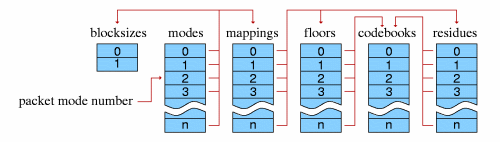
\includegraphics[width=\textwidth]{components}
\captionof{figure}{decoder pipeline configuration}
\end{center}

\subsubsection{Global Config}
Global codec configuration consists of a few audio related fields
(sample rate, channels), Vorbis version (always '0' in Vorbis I),
bitrate hints, and the lists of component instances.  All other
configuration is in the context of specific components.

\subsubsection{Mode}

Each Vorbis frame is coded according to a master 'mode'.  A bitstream
may use one or many modes.

The mode mechanism is used to encode a frame according to one of
multiple possible methods with the intention of choosing a method best
suited to that frame.  Different modes are, e.g. how frame size
is changed from frame to frame. The mode number of a frame serves as a
top level configuration switch for all other specific aspects of frame
decode.

A 'mode' configuration consists of a frame size setting, window type
(always 0, the Vorbis window, in Vorbis I), transform type (always
type 0, the MDCT, in Vorbis I) and a mapping number.  The mapping
number specifies which mapping configuration instance to use for
low-level packet decode and synthesis.


\subsubsection{Mapping}

A mapping contains a channel coupling description and a list of
'submaps' that bundle sets of channel vectors together for grouped
encoding and decoding. These submaps are not references to external
components; the submap list is internal and specific to a mapping.

A 'submap' is a configuration/grouping that applies to a subset of
floor and residue vectors within a mapping.  The submap functions as a
last layer of indirection such that specific special floor or residue
settings can be applied not only to all the vectors in a given mode,
but also specific vectors in a specific mode.  Each submap specifies
the proper floor and residue instance number to use for decoding that
submap's spectral floor and spectral residue vectors.

As an example:

Assume a Vorbis stream that contains six channels in the standard 5.1
format.  The sixth channel, as is normal in 5.1, is bass only.
Therefore it would be wasteful to encode a full-spectrum version of it
as with the other channels.  The submapping mechanism can be used to
apply a full range floor and residue encoding to channels 0 through 4,
and a bass-only representation to the bass channel, thus saving space.
In this example, channels 0-4 belong to submap 0 (which indicates use
of a full-range floor) and channel 5 belongs to submap 1, which uses a
bass-only representation.


\subsubsection{Floor}

Vorbis encodes a spectral 'floor' vector for each PCM channel.  This
vector is a low-resolution representation of the audio spectrum for
the given channel in the current frame, generally used akin to a
whitening filter.  It is named a 'floor' because the Xiph.Org
reference encoder has historically used it as a unit-baseline for
spectral resolution.

A floor encoding may be of two types.  Floor 0 uses a packed LSP
representation on a dB amplitude scale and Bark frequency scale.
Floor 1 represents the curve as a piecewise linear interpolated
representation on a dB amplitude scale and linear frequency scale.
The two floors are semantically interchangeable in
encoding/decoding. However, floor type 1 provides more stable
inter-frame behavior, and so is the preferred choice in all
coupled-stereo and high bitrate modes.  Floor 1 is also considerably
less expensive to decode than floor 0.

Floor 0 is not to be considered deprecated, but it is of limited
modern use.  No known Vorbis encoder past Xiph.Org's own beta 4 makes
use of floor 0.

The values coded/decoded by a floor are both compactly formatted and
make use of entropy coding to save space.  For this reason, a floor
configuration generally refers to multiple codebooks in the codebook
component list.  Entropy coding is thus provided as an abstraction,
and each floor instance may choose from any and all available
codebooks when coding/decoding.


\subsubsection{Residue}
The spectral residue is the fine structure of the audio spectrum
once the floor curve has been subtracted out.  In simplest terms, it
is coded in the bitstream using cascaded (multi-pass) vector
quantization according to one of three specific packing/coding
algorithms numbered 0 through 2.  The packing algorithm details are
configured by residue instance.  As with the floor components, the
final VQ/entropy encoding is provided by external codebook instances
and each residue instance may choose from any and all available
codebooks.

\subsubsection{Codebooks}

Codebooks are a self-contained abstraction that perform entropy
decoding and, optionally, use the entropy-decoded integer value as an
offset into an index of output value vectors, returning the indicated
vector of values.

The entropy coding in a Vorbis I codebook is provided by a standard
Huffman binary tree representation.  This tree is tightly packed using
one of several methods, depending on whether codeword lengths are
ordered or unordered, or the tree is sparse.

The codebook vector index is similarly packed according to index
characteristic.  Most commonly, the vector index is encoded as a
single list of values of possible values that are then permuted into
a list of n-dimensional rows (lattice VQ).



\subsection{High-level Decode Process}

\subsubsection{Decode Setup}

Before decoding can begin, a decoder must initialize using the
bitstream headers matching the stream to be decoded.  Vorbis uses
three header packets; all are required, in-order, by this
specification. Once set up, decode may begin at any audio packet
belonging to the Vorbis stream. In Vorbis I, all packets after the
three initial headers are audio packets.

The header packets are, in order, the identification
header, the comments header, and the setup header.

\paragraph{Identification Header}
The identification header identifies the bitstream as Vorbis, Vorbis
version, and the simple audio characteristics of the stream such as
sample rate and number of channels.

\paragraph{Comment Header}
The comment header includes user text comments (``tags'') and a vendor
string for the application/library that produced the bitstream.  The
encoding and proper use of the comment header is described in \xref{vorbis:spec:comment}.

\paragraph{Setup Header}
The setup header includes extensive CODEC setup information as well as
the complete VQ and Huffman codebooks needed for decode.


\subsubsection{Decode Procedure}

The decoding and synthesis procedure for all audio packets is
fundamentally the same.
\begin{enumerate}
\item decode packet type flag
\item decode mode number
\item decode window shape (long windows only)
\item decode floor
\item decode residue into residue vectors
\item inverse channel coupling of residue vectors
\item generate floor curve from decoded floor data
\item compute dot product of floor and residue, producing audio spectrum vector
\item inverse monolithic transform of audio spectrum vector, always an MDCT in Vorbis I
\item overlap/add left-hand output of transform with right-hand output of previous frame
\item store right hand-data from transform of current frame for future lapping
\item if not first frame, return results of overlap/add as audio result of current frame
\end{enumerate}

Note that clever rearrangement of the synthesis arithmetic is
possible; as an example, one can take advantage of symmetries in the
MDCT to store the right-hand transform data of a partial MDCT for a
50\% inter-frame buffer space savings, and then complete the transform
later before overlap/add with the next frame.  This optimization
produces entirely equivalent output and is naturally perfectly legal.
The decoder must be \emph{entirely mathematically equivalent} to the
specification, it need not be a literal semantic implementation.

\paragraph{Packet type decode}

Vorbis I uses four packet types. The first three packet types mark each
of the three Vorbis headers described above. The fourth packet type
marks an audio packet. All other packet types are reserved; packets
marked with a reserved type should be ignored.

Following the three header packets, all packets in a Vorbis I stream
are audio.  The first step of audio packet decode is to read and
verify the packet type; \emph{a non-audio packet when audio is expected
indicates stream corruption or a non-compliant stream. The decoder
must ignore the packet and not attempt decoding it to
audio}.




\paragraph{Mode decode}
Vorbis allows an encoder to set up multiple, numbered packet 'modes',
as described earlier, all of which may be used in a given Vorbis
stream. The mode is encoded as an integer used as a direct offset into
the mode instance index.


\paragraph{Window shape decode (long windows only)} \label{vorbis:spec:window}

Vorbis frames may be one of two PCM sample sizes specified during
codec setup.  In Vorbis I, legal frame sizes are powers of two from 64
to 8192 samples.  Aside from coupling, Vorbis handles channels as
independent vectors and these frame sizes are in samples per channel.

Vorbis uses an overlapping transform, namely the MDCT, to blend one
frame into the next, avoiding most inter-frame block boundary
artifacts.  The MDCT output of one frame is windowed according to MDCT
requirements, overlapped 50\% with the output of the previous frame and
added.  The window shape assures seamless reconstruction.

This is easy to visualize in the case of equal sized-windows:

\begin{center}
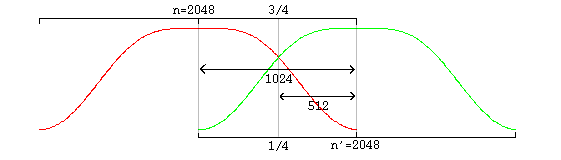
\includegraphics[width=\textwidth]{window1}
\captionof{figure}{overlap of two equal-sized windows}
\end{center}

And slightly more complex in the case of overlapping unequal sized
windows:

\begin{center}
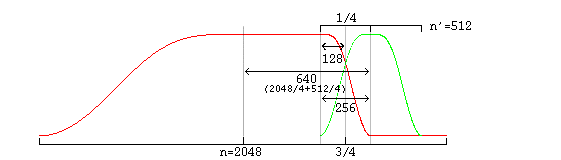
\includegraphics[width=\textwidth]{window2}
\captionof{figure}{overlap of a long and a short window}
\end{center}

In the unequal-sized window case, the window shape of the long window
must be modified for seamless lapping as above.  It is possible to
correctly infer window shape to be applied to the current window from
knowing the sizes of the current, previous and next window.  It is
legal for a decoder to use this method. However, in the case of a long
window (short windows require no modification), Vorbis also codes two
flag bits to specify pre- and post- window shape.  Although not
strictly necessary for function, this minor redundancy allows a packet
to be fully decoded to the point of lapping entirely independently of
any other packet, allowing easier abstraction of decode layers as well
as allowing a greater level of easy parallelism in encode and
decode.

A description of valid window functions for use with an inverse MDCT
can be found in \cite{Sporer/Brandenburg/Edler}.  Vorbis windows
all use the slope function
\[ y = \sin(.5*\pi \, \sin^2((x+.5)/n*\pi)) . \]



\paragraph{floor decode}
Each floor is encoded/decoded in channel order, however each floor
belongs to a 'submap' that specifies which floor configuration to
use.  All floors are decoded before residue decode begins.


\paragraph{residue decode}

Although the number of residue vectors equals the number of channels,
channel coupling may mean that the raw residue vectors extracted
during decode do not map directly to specific channels.  When channel
coupling is in use, some vectors will correspond to coupled magnitude
or angle.  The coupling relationships are described in the codec setup
and may differ from frame to frame, due to different mode numbers.

Vorbis codes residue vectors in groups by submap; the coding is done
in submap order from submap 0 through n-1.  This differs from floors
which are coded using a configuration provided by submap number, but
are coded individually in channel order.



\paragraph{inverse channel coupling}

A detailed discussion of stereo in the Vorbis codec can be found in
the document \href{stereo.html}{Stereo Channel Coupling in the
Vorbis CODEC}.  Vorbis is not limited to only stereo coupling, but
the stereo document also gives a good overview of the generic coupling
mechanism.

Vorbis coupling applies to pairs of residue vectors at a time;
decoupling is done in-place a pair at a time in the order and using
the vectors specified in the current mapping configuration.  The
decoupling operation is the same for all pairs, converting square
polar representation (where one vector is magnitude and the second
angle) back to Cartesian representation.

After decoupling, in order, each pair of vectors on the coupling list,
the resulting residue vectors represent the fine spectral detail
of each output channel.



\paragraph{generate floor curve}

The decoder may choose to generate the floor curve at any appropriate
time.  It is reasonable to generate the output curve when the floor
data is decoded from the raw packet, or it can be generated after
inverse coupling and applied to the spectral residue directly,
combining generation and the dot product into one step and eliminating
some working space.

Both floor 0 and floor 1 generate a linear-range, linear-domain output
vector to be multiplied (dot product) by the linear-range,
linear-domain spectral residue.



\paragraph{compute floor/residue dot product}

This step is straightforward; for each output channel, the decoder
multiplies the floor curve and residue vectors element by element,
producing the finished audio spectrum of each channel.

% TODO/FIXME: The following two paragraphs have identical twins
%   in section 4 (under "dot product")
One point is worth mentioning about this dot product; a common mistake
in a fixed point implementation might be to assume that a 32 bit
fixed-point representation for floor and residue and direct
multiplication of the vectors is sufficient for acceptable spectral
depth in all cases because it happens to mostly work with the current
Xiph.Org reference encoder.

However, floor vector values can span \~{}140dB (\~{}24 bits unsigned), and
the audio spectrum vector should represent a minimum of 120dB (\~{}21
bits with sign), even when output is to a 16 bit PCM device.  For the
residue vector to represent full scale if the floor is nailed to
$-140$dB, it must be able to span 0 to $+140$dB.  For the residue vector
to reach full scale if the floor is nailed at 0dB, it must be able to
represent $-140$dB to $+0$dB.  Thus, in order to handle full range
dynamics, a residue vector may span $-140$dB to $+140$dB entirely within
spec.  A 280dB range is approximately 48 bits with sign; thus the
residue vector must be able to represent a 48 bit range and the dot
product must be able to handle an effective 48 bit times 24 bit
multiplication.  This range may be achieved using large (64 bit or
larger) integers, or implementing a movable binary point
representation.



\paragraph{inverse monolithic transform (MDCT)}

The audio spectrum is converted back into time domain PCM audio via an
inverse Modified Discrete Cosine Transform (MDCT).  A detailed
description of the MDCT is available in \cite{Sporer/Brandenburg/Edler}.

Note that the PCM produced directly from the MDCT is not yet finished
audio; it must be lapped with surrounding frames using an appropriate
window (such as the Vorbis window) before the MDCT can be considered
orthogonal.



\paragraph{overlap/add data}
Windowed MDCT output is overlapped and added with the right hand data
of the previous window such that the 3/4 point of the previous window
is aligned with the 1/4 point of the current window (as illustrated in
the window overlap diagram). At this point, the audio data between the
center of the previous frame and the center of the current frame is
now finished and ready to be returned.


\paragraph{cache right hand data}
The decoder must cache the right hand portion of the current frame to
be lapped with the left hand portion of the next frame.



\paragraph{return finished audio data}

The overlapped portion produced from overlapping the previous and
current frame data is finished data to be returned by the decoder.
This data spans from the center of the previous window to the center
of the current window.  In the case of same-sized windows, the amount
of data to return is one-half block consisting of and only of the
overlapped portions. When overlapping a short and long window, much of
the returned range is not actually overlap.  This does not damage
transform orthogonality.  Pay attention however to returning the
correct data range; the amount of data to be returned is:

\begin{Verbatim}[commandchars=\\\{\}]
window\_blocksize(previous\_window)/4+window\_blocksize(current\_window)/4
\end{Verbatim}

from the center of the previous window to the center of the current
window.

Data is not returned from the first frame; it must be used to 'prime'
the decode engine.  The encoder accounts for this priming when
calculating PCM offsets; after the first frame, the proper PCM output
offset is '0' (as no data has been returned yet).

% -*- mode: latex; TeX-master: "Vorbis_I_spec"; -*-
%!TEX root = Vorbis_I_spec.tex
% $Id$
\section{Bitpacking Convention} \label{vorbis:spec:bitpacking}

\subsection{Overview}

The Vorbis codec uses relatively unstructured raw packets containing
arbitrary-width binary integer fields.  Logically, these packets are a
bitstream in which bits are coded one-by-one by the encoder and then
read one-by-one in the same monotonically increasing order by the
decoder.  Most current binary storage arrangements group bits into a
native word size of eight bits (octets), sixteen bits, thirty-two bits
or, less commonly other fixed word sizes.  The Vorbis bitpacking
convention specifies the correct mapping of the logical packet
bitstream into an actual representation in fixed-width words.


\subsubsection{octets, bytes and words}

In most contemporary architectures, a 'byte' is synonymous with an
'octet', that is, eight bits.  This has not always been the case;
seven, ten, eleven and sixteen bit 'bytes' have been used.  For
purposes of the bitpacking convention, a byte implies the native,
smallest integer storage representation offered by a platform.  On
modern platforms, this is generally assumed to be eight bits (not
necessarily because of the processor but because of the
filesystem/memory architecture.  Modern filesystems invariably offer
bytes as the fundamental atom of storage).  A 'word' is an integer
size that is a grouped multiple of this smallest size.

The most ubiquitous architectures today consider a 'byte' to be an
octet (eight bits) and a word to be a group of two, four or eight
bytes (16, 32 or 64 bits).  Note however that the Vorbis bitpacking
convention is still well defined for any native byte size; Vorbis uses
the native bit-width of a given storage system. This document assumes
that a byte is one octet for purposes of example.

\subsubsection{bit order}

A byte has a well-defined 'least significant' bit (LSb), which is the
only bit set when the byte is storing the two's complement integer
value +1.  A byte's 'most significant' bit (MSb) is at the opposite
end of the byte. Bits in a byte are numbered from zero at the LSb to
$n$ ($n=7$ in an octet) for the
MSb.



\subsubsection{byte order}

Words are native groupings of multiple bytes.  Several byte orderings
are possible in a word; the common ones are 3-2-1-0 ('big endian' or
'most significant byte first' in which the highest-valued byte comes
first), 0-1-2-3 ('little endian' or 'least significant byte first' in
which the lowest value byte comes first) and less commonly 3-1-2-0 and
0-2-1-3 ('mixed endian').

The Vorbis bitpacking convention specifies storage and bitstream
manipulation at the byte, not word, level, thus host word ordering is
of a concern only during optimization when writing high performance
code that operates on a word of storage at a time rather than by byte.
Logically, bytes are always coded and decoded in order from byte zero
through byte $n$.



\subsubsection{coding bits into byte sequences}

The Vorbis codec has need to code arbitrary bit-width integers, from
zero to 32 bits wide, into packets.  These integer fields are not
aligned to the boundaries of the byte representation; the next field
is written at the bit position at which the previous field ends.

The encoder logically packs integers by writing the LSb of a binary
integer to the logical bitstream first, followed by next least
significant bit, etc, until the requested number of bits have been
coded.  When packing the bits into bytes, the encoder begins by
placing the LSb of the integer to be written into the least
significant unused bit position of the destination byte, followed by
the next-least significant bit of the source integer and so on up to
the requested number of bits.  When all bits of the destination byte
have been filled, encoding continues by zeroing all bits of the next
byte and writing the next bit into the bit position 0 of that byte.
Decoding follows the same process as encoding, but by reading bits
from the byte stream and reassembling them into integers.



\subsubsection{signedness}

The signedness of a specific number resulting from decode is to be
interpreted by the decoder given decode context.  That is, the three
bit binary pattern 'b111' can be taken to represent either 'seven' as
an unsigned integer, or '-1' as a signed, two's complement integer.
The encoder and decoder are responsible for knowing if fields are to
be treated as signed or unsigned.



\subsubsection{coding example}

Code the 4 bit integer value '12' [b1100] into an empty bytestream.
Bytestream result:

\begin{Verbatim}[commandchars=\\\{\}]
              |
              V

        7 6 5 4 3 2 1 0
byte 0 [0 0 0 0 1 1 0 0]  <-
byte 1 [               ]
byte 2 [               ]
byte 3 [               ]
             ...
byte n [               ]  bytestream length == 1 byte

\end{Verbatim}


Continue by coding the 3 bit integer value '-1' [b111]:

\begin{Verbatim}[commandchars=\\\{\}]
        |
        V

        7 6 5 4 3 2 1 0
byte 0 [0 1 1 1 1 1 0 0]  <-
byte 1 [               ]
byte 2 [               ]
byte 3 [               ]
             ...
byte n [               ]  bytestream length == 1 byte
\end{Verbatim}


Continue by coding the 7 bit integer value '17' [b0010001]:

\begin{Verbatim}[commandchars=\\\{\}]
          |
          V

        7 6 5 4 3 2 1 0
byte 0 [1 1 1 1 1 1 0 0]
byte 1 [0 0 0 0 1 0 0 0]  <-
byte 2 [               ]
byte 3 [               ]
             ...
byte n [               ]  bytestream length == 2 bytes
                          bit cursor == 6
\end{Verbatim}


Continue by coding the 13 bit integer value '6969' [b110 11001110 01]:

\begin{Verbatim}[commandchars=\\\{\}]
                |
                V

        7 6 5 4 3 2 1 0
byte 0 [1 1 1 1 1 1 0 0]
byte 1 [0 1 0 0 1 0 0 0]
byte 2 [1 1 0 0 1 1 1 0]
byte 3 [0 0 0 0 0 1 1 0]  <-
             ...
byte n [               ]  bytestream length == 4 bytes

\end{Verbatim}




\subsubsection{decoding example}

Reading from the beginning of the bytestream encoded in the above example:

\begin{Verbatim}[commandchars=\\\{\}]
                      |
                      V

        7 6 5 4 3 2 1 0
byte 0 [1 1 1 1 1 1 0 0]  <-
byte 1 [0 1 0 0 1 0 0 0]
byte 2 [1 1 0 0 1 1 1 0]
byte 3 [0 0 0 0 0 1 1 0]  bytestream length == 4 bytes

\end{Verbatim}


We read two, two-bit integer fields, resulting in the returned numbers
'b00' and 'b11'.  Two things are worth noting here:

\begin{itemize}
\item Although these four bits were originally written as a single
four-bit integer, reading some other combination of bit-widths from the
bitstream is well defined.  There are no artificial alignment
boundaries maintained in the bitstream.

\item The second value is the
two-bit-wide integer 'b11'.  This value may be interpreted either as
the unsigned value '3', or the signed value '-1'.  Signedness is
dependent on decode context.
\end{itemize}




\subsubsection{end-of-packet alignment}

The typical use of bitpacking is to produce many independent
byte-aligned packets which are embedded into a larger byte-aligned
container structure, such as an Ogg transport bitstream.  Externally,
each bytestream (encoded bitstream) must begin and end on a byte
boundary.  Often, the encoded bitstream is not an integer number of
bytes, and so there is unused (uncoded) space in the last byte of a
packet.

Unused space in the last byte of a bytestream is always zeroed during
the coding process.  Thus, should this unused space be read, it will
return binary zeroes.

Attempting to read past the end of an encoded packet results in an
'end-of-packet' condition.  End-of-packet is not to be considered an
error; it is merely a state indicating that there is insufficient
remaining data to fulfill the desired read size.  Vorbis uses truncated
packets as a normal mode of operation, and as such, decoders must
handle reading past the end of a packet as a typical mode of
operation. Any further read operations after an 'end-of-packet'
condition shall also return 'end-of-packet'.



\subsubsection{reading zero bits}

Reading a zero-bit-wide integer returns the value '0' and does not
increment the stream cursor.  Reading to the end of the packet (but
not past, such that an 'end-of-packet' condition has not triggered)
and then reading a zero bit integer shall succeed, returning 0, and
not trigger an end-of-packet condition.  Reading a zero-bit-wide
integer after a previous read sets 'end-of-packet' shall also fail
with 'end-of-packet'.







% -*- mode: latex; TeX-master: "Vorbis_I_spec"; -*-
%!TEX root = Vorbis_I_spec.tex
% $Id$
\section{Probability Model and Codebooks} \label{vorbis:spec:codebook}

\subsection{Overview}

Unlike practically every other mainstream audio codec, Vorbis has no
statically configured probability model, instead packing all entropy
decoding configuration, VQ and Huffman, into the bitstream itself in
the third header, the codec setup header.  This packed configuration
consists of multiple 'codebooks', each containing a specific
Huffman-equivalent representation for decoding compressed codewords as
well as an optional lookup table of output vector values to which a
decoded Huffman value is applied as an offset, generating the final
decoded output corresponding to a given compressed codeword.

\subsubsection{Bitwise operation}
The codebook mechanism is built on top of the vorbis bitpacker. Both
the codebooks themselves and the codewords they decode are unrolled
from a packet as a series of arbitrary-width values read from the
stream according to \xref{vorbis:spec:bitpacking}.




\subsection{Packed codebook format}

For purposes of the examples below, we assume that the storage
system's native byte width is eight bits.  This is not universally
true; see \xref{vorbis:spec:bitpacking} for discussion
relating to non-eight-bit bytes.

\subsubsection{codebook decode}

A codebook begins with a 24 bit sync pattern, 0x564342:

\begin{Verbatim}[commandchars=\\\{\}]
byte 0: [ 0 1 0 0 0 0 1 0 ] (0x42)
byte 1: [ 0 1 0 0 0 0 1 1 ] (0x43)
byte 2: [ 0 1 0 1 0 1 1 0 ] (0x56)
\end{Verbatim}

16 bit \varname{[codebook\_dimensions]} and 24 bit \varname{[codebook\_entries]} fields:

\begin{Verbatim}[commandchars=\\\{\}]

byte 3: [ X X X X X X X X ]
byte 4: [ X X X X X X X X ] [codebook\_dimensions] (16 bit unsigned)

byte 5: [ X X X X X X X X ]
byte 6: [ X X X X X X X X ]
byte 7: [ X X X X X X X X ] [codebook\_entries] (24 bit unsigned)

\end{Verbatim}

Next is the \varname{[ordered]} bit flag:

\begin{Verbatim}[commandchars=\\\{\}]

byte 8: [               X ] [ordered] (1 bit)

\end{Verbatim}

Each entry, numbering a
total of \varname{[codebook\_entries]}, is assigned a codeword length.
We now read the list of codeword lengths and store these lengths in
the array \varname{[codebook\_codeword\_lengths]}. Decode of lengths is
according to whether the \varname{[ordered]} flag is set or unset.

\begin{itemize}
\item
  If the \varname{[ordered]} flag is unset, the codeword list is not
  length ordered and the decoder needs to read each codeword length
  one-by-one.

  The decoder first reads one additional bit flag, the
  \varname{[sparse]} flag.  This flag determines whether or not the
  codebook contains unused entries that are not to be included in the
  codeword decode tree:

\begin{Verbatim}[commandchars=\\\{\}]
byte 8: [             X 1 ] [sparse] flag (1 bit)
\end{Verbatim}

  The decoder now performs for each of the \varname{[codebook\_entries]}
  codebook entries:

\begin{Verbatim}[commandchars=\\\{\}]

  1) if([sparse] is set) \{

         2) [flag] = read one bit;
         3) if([flag] is set) \{

              4) [length] = read a five bit unsigned integer;
              5) codeword length for this entry is [length]+1;

            \} else \{

              6) this entry is unused.  mark it as such.

            \}

     \} else the sparse flag is not set \{

        7) [length] = read a five bit unsigned integer;
        8) the codeword length for this entry is [length]+1;

     \}

\end{Verbatim}

\item
  If the \varname{[ordered]} flag is set, the codeword list for this
  codebook is encoded in ascending length order.  Rather than reading
  a length for every codeword, the encoder reads the number of
  codewords per length.  That is, beginning at entry zero:

\begin{Verbatim}[commandchars=\\\{\}]
  1) [current\_entry] = 0;
  2) [current\_length] = read a five bit unsigned integer and add 1;
  3) [number] = read \link{vorbis:spec:ilog}{ilog}([codebook\_entries] - [current\_entry]) bits as an unsigned integer
  4) set the entries [current\_entry] through [current\_entry]+[number]-1, inclusive,
    of the [codebook\_codeword\_lengths] array to [current\_length]
  5) set [current\_entry] to [number] + [current\_entry]
  6) increment [current\_length] by 1
  7) if [current\_entry] is greater than [codebook\_entries] ERROR CONDITION;
    the decoder will not be able to read this stream.
  8) if [current\_entry] is less than [codebook\_entries], repeat process starting at 3)
  9) done.
\end{Verbatim}

\end{itemize}

After all codeword lengths have been decoded, the decoder reads the
vector lookup table.  Vorbis I supports three lookup types:
\begin{enumerate}
\item
No lookup
\item
Implicitly populated value mapping (lattice VQ)
\item
Explicitly populated value mapping (tessellated or 'foam'
VQ)
\end{enumerate}


The lookup table type is read as a four bit unsigned integer:
\begin{Verbatim}[commandchars=\\\{\}]
  1) [codebook\_lookup\_type] = read four bits as an unsigned integer
\end{Verbatim}

Codebook decode precedes according to \varname{[codebook\_lookup\_type]}:
\begin{itemize}
\item
Lookup type zero indicates no lookup to be read.  Proceed past
lookup decode.
\item
Lookup types one and two are similar, differing only in the
number of lookup values to be read.  Lookup type one reads a list of
values that are permuted in a set pattern to build a list of vectors,
each vector of order \varname{[codebook\_dimensions]} scalars.  Lookup
type two builds the same vector list, but reads each scalar for each
vector explicitly, rather than building vectors from a smaller list of
possible scalar values.  Lookup decode proceeds as follows:

\begin{Verbatim}[commandchars=\\\{\}]
  1) [codebook\_minimum\_value] = \link{vorbis:spec:float32:unpack}{float32\_unpack}( read 32 bits as an unsigned integer)
  2) [codebook\_delta\_value] = \link{vorbis:spec:float32:unpack}{float32\_unpack}( read 32 bits as an unsigned integer)
  3) [codebook\_value\_bits] = read 4 bits as an unsigned integer and add 1
  4) [codebook\_sequence\_p] = read 1 bit as a boolean flag

  if ( [codebook\_lookup\_type] is 1 ) \{

     5) [codebook\_lookup\_values] = \link{vorbis:spec:lookup1:values}{lookup1\_values}(\varname{[codebook\_entries]}, \varname{[codebook\_dimensions]} )

  \} else \{

     6) [codebook\_lookup\_values] = \varname{[codebook\_entries]} * \varname{[codebook\_dimensions]}

  \}

  7) read a total of [codebook\_lookup\_values] unsigned integers of [codebook\_value\_bits] each;
     store these in order in the array [codebook\_multiplicands]
\end{Verbatim}
\item
A \varname{[codebook\_lookup\_type]} of greater than two is reserved
and indicates a stream that is not decodable by the specification in this
document.

\end{itemize}


An 'end of packet' during any read operation in the above steps is
considered an error condition rendering the stream undecodable.

\paragraph{Huffman decision tree representation}

The \varname{[codebook\_codeword\_lengths]} array and
\varname{[codebook\_entries]} value uniquely define the Huffman decision
tree used for entropy decoding.

Briefly, each used codebook entry (recall that length-unordered
codebooks support unused codeword entries) is assigned, in order, the
lowest valued unused binary Huffman codeword possible.  Assume the
following codeword length list:

\begin{Verbatim}[commandchars=\\\{\}]
entry 0: length 2
entry 1: length 4
entry 2: length 4
entry 3: length 4
entry 4: length 4
entry 5: length 2
entry 6: length 3
entry 7: length 3
\end{Verbatim}

Assigning codewords in order (lowest possible value of the appropriate
length to highest) results in the following codeword list:

\begin{Verbatim}[commandchars=\\\{\}]
entry 0: length 2 codeword 00
entry 1: length 4 codeword 0100
entry 2: length 4 codeword 0101
entry 3: length 4 codeword 0110
entry 4: length 4 codeword 0111
entry 5: length 2 codeword 10
entry 6: length 3 codeword 110
entry 7: length 3 codeword 111
\end{Verbatim}


\begin{note}
Unlike most binary numerical values in this document, we
intend the above codewords to be read and used bit by bit from left to
right, thus the codeword '001' is the bit string 'zero, zero, one'.
When determining 'lowest possible value' in the assignment definition
above, the leftmost bit is the MSb.
\end{note}

It is clear that the codeword length list represents a Huffman
decision tree with the entry numbers equivalent to the leaves numbered
left-to-right:

\begin{center}
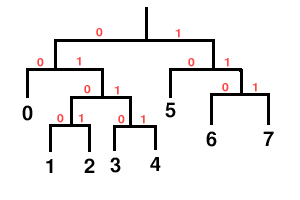
\includegraphics[width=10cm]{hufftree}
\captionof{figure}{huffman tree illustration}
\end{center}


As we assign codewords in order, we see that each choice constructs a
new leaf in the leftmost possible position.

Note that it's possible to underspecify or overspecify a Huffman tree
via the length list.  In the above example, if codeword seven were
eliminated, it's clear that the tree is unfinished:

\begin{center}
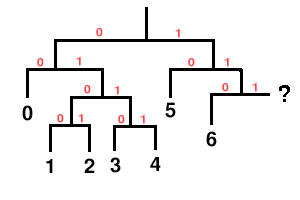
\includegraphics[width=10cm]{hufftree-under}
\captionof{figure}{underspecified huffman tree illustration}
\end{center}


Similarly, in the original codebook, it's clear that the tree is fully
populated and a ninth codeword is impossible.  Both underspecified and
overspecified trees are an error condition rendering the stream
undecodable. Take special care that a codebook with a single used
entry is handled properly; it consists of a single codework of zero
bits and 'reading' a value out of such a codebook always returns the
single used value and sinks zero bits.  

Codebook entries marked 'unused' are simply skipped in the assigning
process.  They have no codeword and do not appear in the decision
tree, thus it's impossible for any bit pattern read from the stream to
decode to that entry number.



\paragraph{VQ lookup table vector representation}

Unpacking the VQ lookup table vectors relies on the following values:
\begin{programlisting}
the [codebook\_multiplicands] array
[codebook\_minimum\_value]
[codebook\_delta\_value]
[codebook\_sequence\_p]
[codebook\_lookup\_type]
[codebook\_entries]
[codebook\_dimensions]
[codebook\_lookup\_values]
\end{programlisting}

\bigskip

Decoding (unpacking) a specific vector in the vector lookup table
proceeds according to \varname{[codebook\_lookup\_type]}.  The unpacked
vector values are what a codebook would return during audio packet
decode in a VQ context.

\paragraph{Vector value decode: Lookup type 1}

Lookup type one specifies a lattice VQ lookup table built
algorithmically from a list of scalar values.  Calculate (unpack) the
final values of a codebook entry vector from the entries in
\varname{[codebook\_multiplicands]} as follows (\varname{[value\_vector]}
is the output vector representing the vector of values for entry number
\varname{[lookup\_offset]} in this codebook):

\begin{Verbatim}[commandchars=\\\{\}]
  1) [last] = 0;
  2) [index\_divisor] = 1;
  3) iterate [i] over the range 0 ... [codebook\_dimensions]-1 (once for each scalar value in the value vector) \{

       4) [multiplicand\_offset] = ( [lookup\_offset] divided by [index\_divisor] using integer
          division ) integer modulo [codebook\_lookup\_values]

       5) vector [value\_vector] element [i] =
            ( [codebook\_multiplicands] array element number [multiplicand\_offset] ) *
            [codebook\_delta\_value] + [codebook\_minimum\_value] + [last];

       6) if ( [codebook\_sequence\_p] is set ) then set [last] = vector [value\_vector] element [i]

       7) [index\_divisor] = [index\_divisor] * [codebook\_lookup\_values]

     \}

  8) vector calculation completed.
\end{Verbatim}



\paragraph{Vector value decode: Lookup type 2}

Lookup type two specifies a VQ lookup table in which each scalar in
each vector is explicitly set by the \varname{[codebook\_multiplicands]}
array in a one-to-one mapping.  Calculate [unpack] the
final values of a codebook entry vector from the entries in
\varname{[codebook\_multiplicands]} as follows (\varname{[value\_vector]}
is the output vector representing the vector of values for entry number
\varname{[lookup\_offset]} in this codebook):

\begin{Verbatim}[commandchars=\\\{\}]
  1) [last] = 0;
  2) [multiplicand\_offset] = [lookup\_offset] * [codebook\_dimensions]
  3) iterate [i] over the range 0 ... [codebook\_dimensions]-1 (once for each scalar value in the value vector) \{

       4) vector [value\_vector] element [i] =
            ( [codebook\_multiplicands] array element number [multiplicand\_offset] ) *
            [codebook\_delta\_value] + [codebook\_minimum\_value] + [last];

       5) if ( [codebook\_sequence\_p] is set ) then set [last] = vector [value\_vector] element [i]

       6) increment [multiplicand\_offset]

     \}

  7) vector calculation completed.
\end{Verbatim}









\subsection{Use of the codebook abstraction}

The decoder uses the codebook abstraction much as it does the
bit-unpacking convention; a specific codebook reads a
codeword from the bitstream, decoding it into an entry number, and then
returns that entry number to the decoder (when used in a scalar
entropy coding context), or uses that entry number as an offset into
the VQ lookup table, returning a vector of values (when used in a context
desiring a VQ value). Scalar or VQ context is always explicit; any call
to the codebook mechanism requests either a scalar entry number or a
lookup vector.

Note that VQ lookup type zero indicates that there is no lookup table;
requesting decode using a codebook of lookup type 0 in any context
expecting a vector return value (even in a case where a vector of
dimension one) is forbidden.  If decoder setup or decode requests such
an action, that is an error condition rendering the packet
undecodable.

Using a codebook to read from the packet bitstream consists first of
reading and decoding the next codeword in the bitstream. The decoder
reads bits until the accumulated bits match a codeword in the
codebook.  This process can be though of as logically walking the
Huffman decode tree by reading one bit at a time from the bitstream,
and using the bit as a decision boolean to take the 0 branch (left in
the above examples) or the 1 branch (right in the above examples).
Walking the tree finishes when the decode process hits a leaf in the
decision tree; the result is the entry number corresponding to that
leaf.  Reading past the end of a packet propagates the 'end-of-stream'
condition to the decoder.

When used in a scalar context, the resulting codeword entry is the
desired return value.

When used in a VQ context, the codeword entry number is used as an
offset into the VQ lookup table.  The value returned to the decoder is
the vector of scalars corresponding to this offset.


% -*- mode: latex; TeX-master: "Vorbis_I_spec"; -*-
%!TEX root = Vorbis_I_spec.tex
% $Id$
\section{Codec Setup and Packet Decode} \label{vorbis:spec:codec}

\subsection{Overview}

This document serves as the top-level reference document for the
bit-by-bit decode specification of Vorbis I.  This document assumes a
high-level understanding of the Vorbis decode process, which is
provided in \xref{vorbis:spec:intro}.  \xref{vorbis:spec:bitpacking} covers reading and writing bit fields from
and to bitstream packets.



\subsection{Header decode and decode setup}

A Vorbis bitstream begins with three header packets. The header
packets are, in order, the identification header, the comments header,
and the setup header. All are required for decode compliance.  An
end-of-packet condition during decoding the first or third header
packet renders the stream undecodable.  End-of-packet decoding the
comment header is a non-fatal error condition.

\subsubsection{Common header decode}

Each header packet begins with the same header fields.


\begin{Verbatim}[commandchars=\\\{\}]
  1) [packet\_type] : 8 bit value
  2) 0x76, 0x6f, 0x72, 0x62, 0x69, 0x73: the characters 'v','o','r','b','i','s' as six octets
\end{Verbatim}

Decode continues according to packet type; the identification header
is type 1, the comment header type 3 and the setup header type 5
(these types are all odd as a packet with a leading single bit of '0'
is an audio packet).  The packets must occur in the order of
identification, comment, setup.



\subsubsection{Identification header}

The identification header is a short header of only a few fields used
to declare the stream definitively as Vorbis, and provide a few externally
relevant pieces of information about the audio stream. The
identification header is coded as follows:

\begin{Verbatim}[commandchars=\\\{\}]
 1) [vorbis\_version] = read 32 bits as unsigned integer
 2) [audio\_channels] = read 8 bit integer as unsigned
 3) [audio\_sample\_rate] = read 32 bits as unsigned integer
 4) [bitrate\_maximum] = read 32 bits as signed integer
 5) [bitrate\_nominal] = read 32 bits as signed integer
 6) [bitrate\_minimum] = read 32 bits as signed integer
 7) [blocksize\_0] = 2 exponent (read 4 bits as unsigned integer)
 8) [blocksize\_1] = 2 exponent (read 4 bits as unsigned integer)
 9) [framing\_flag] = read one bit
\end{Verbatim}

\varname{[vorbis\_version]} is to read '0' in order to be compatible
with this document.  Both \varname{[audio\_channels]} and
\varname{[audio\_sample\_rate]} must read greater than zero.  Allowed final
blocksize values are 64, 128, 256, 512, 1024, 2048, 4096 and 8192 in
Vorbis I.  \varname{[blocksize\_0]} must be less than or equal to
\varname{[blocksize\_1]}.  The framing bit must be nonzero.  Failure to
meet any of these conditions renders a stream undecodable.

The bitrate fields above are used only as hints. The nominal bitrate
field especially may be considerably off in purely VBR streams.  The
fields are meaningful only when greater than zero.

\begin{itemize}
  \item All three fields set to the same value implies a fixed rate, or tightly bounded, nearly fixed-rate bitstream
  \item Only nominal set implies a VBR or ABR stream that averages the nominal bitrate
  \item Maximum and or minimum set implies a VBR bitstream that obeys the bitrate limits
  \item None set indicates the encoder does not care to speculate.
\end{itemize}




\subsubsection{Comment header}
Comment header decode and data specification is covered in
\xref{vorbis:spec:comment}.


\subsubsection{Setup header}

Vorbis codec setup is configurable to an extreme degree:

\begin{center}
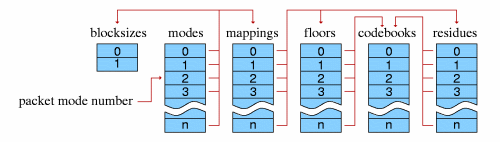
\includegraphics[width=\textwidth]{components}
\captionof{figure}{decoder pipeline configuration}
\end{center}


The setup header contains the bulk of the codec setup information
needed for decode.  The setup header contains, in order, the lists of
codebook configurations, time-domain transform configurations
(placeholders in Vorbis I), floor configurations, residue
configurations, channel mapping configurations and mode
configurations. It finishes with a framing bit of '1'.  Header decode
proceeds in the following order:

\paragraph{Codebooks}

\begin{enumerate}
\item \varname{[vorbis\_codebook\_count]} = read eight bits as unsigned integer and add one
\item Decode \varname{[vorbis\_codebook\_count]} codebooks in order as defined
in \xref{vorbis:spec:codebook}.  Save each configuration, in
order, in an array of
codebook configurations \varname{[vorbis\_codebook\_configurations]}.
\end{enumerate}



\paragraph{Time domain transforms}

These hooks are placeholders in Vorbis I.  Nevertheless, the
configuration placeholder values must be read to maintain bitstream
sync.

\begin{enumerate}
\item \varname{[vorbis\_time\_count]} = read 6 bits as unsigned integer and add one
\item read \varname{[vorbis\_time\_count]} 16 bit values; each value should be zero.  If any value is nonzero, this is an error condition and the stream is undecodable.
\end{enumerate}



\paragraph{Floors}

Vorbis uses two floor types; header decode is handed to the decode
abstraction of the appropriate type.

\begin{enumerate}
 \item \varname{[vorbis\_floor\_count]} = read 6 bits as unsigned integer and add one
 \item For each \varname{[i]} of \varname{[vorbis\_floor\_count]} floor numbers:
  \begin{enumerate}
   \item read the floor type: vector \varname{[vorbis\_floor\_types]} element \varname{[i]} =
read 16 bits as unsigned integer
   \item If the floor type is zero, decode the floor
configuration as defined in \xref{vorbis:spec:floor0}; save
this
configuration in slot \varname{[i]} of the floor configuration array \varname{[vorbis\_floor\_configurations]}.
   \item If the floor type is one,
decode the floor configuration as defined in \xref{vorbis:spec:floor1}; save this configuration in slot \varname{[i]} of the floor configuration array \varname{[vorbis\_floor\_configurations]}.
   \item If the the floor type is greater than one, this stream is undecodable; ERROR CONDITION
  \end{enumerate}

\end{enumerate}



\paragraph{Residues}

Vorbis uses three residue types; header decode of each type is identical.


\begin{enumerate}
\item \varname{[vorbis\_residue\_count]} = read 6 bits as unsigned integer and add one

\item For each of \varname{[vorbis\_residue\_count]} residue numbers:
 \begin{enumerate}
  \item read the residue type; vector \varname{[vorbis\_residue\_types]} element \varname{[i]} = read 16 bits as unsigned integer
  \item If the residue type is zero,
one or two, decode the residue configuration as defined in \xref{vorbis:spec:residue}; save this configuration in slot \varname{[i]} of the residue configuration array \varname{[vorbis\_residue\_configurations]}.
  \item If the the residue type is greater than two, this stream is undecodable; ERROR CONDITION
 \end{enumerate}

\end{enumerate}



\paragraph{Mappings}

Mappings are used to set up specific pipelines for encoding
multichannel audio with varying channel mapping applications. Vorbis I
uses a single mapping type (0), with implicit PCM channel mappings.

% FIXME/TODO: LaTeX cannot nest enumerate that deeply, so I have to use
% itemize at the innermost level. However, it would be much better to 
% rewrite this pseudocode using listings or algoritmicx or some other
% package geared towards this.
\begin{enumerate}
 \item \varname{[vorbis\_mapping\_count]} = read 6 bits as unsigned integer and add one
 \item For each \varname{[i]} of \varname{[vorbis\_mapping\_count]} mapping numbers:
  \begin{enumerate}
   \item read the mapping type: 16 bits as unsigned integer.  There's no reason to save the mapping type in Vorbis I.
   \item If the mapping type is nonzero, the stream is undecodable
   \item If the mapping type is zero:
    \begin{enumerate}
     \item read 1 bit as a boolean flag
      \begin{enumerate}
       \item if set, \varname{[vorbis\_mapping\_submaps]} = read 4 bits as unsigned integer and add one
       \item if unset, \varname{[vorbis\_mapping\_submaps]} = 1
      \end{enumerate}


     \item read 1 bit as a boolean flag
       \begin{enumerate}
         \item if set, square polar channel mapping is in use:
           \begin{itemize}
             \item \varname{[vorbis\_mapping\_coupling\_steps]} = read 8 bits as unsigned integer and add one
             \item for \varname{[j]} each of \varname{[vorbis\_mapping\_coupling\_steps]} steps:
               \begin{itemize}
                 \item vector \varname{[vorbis\_mapping\_magnitude]} element \varname{[j]}= read \link{vorbis:spec:ilog}{ilog}(\varname{[audio\_channels]} - 1) bits as unsigned integer
                 \item vector \varname{[vorbis\_mapping\_angle]} element \varname{[j]}= read \link{vorbis:spec:ilog}{ilog}(\varname{[audio\_channels]} - 1) bits as unsigned integer
                 \item the numbers read in the above two steps are channel numbers representing the channel to treat as magnitude and the channel to treat as angle, respectively.  If for any coupling step the angle channel number equals the magnitude channel number, the magnitude channel number is greater than \varname{[audio\_channels]}-1, or the angle channel is greater than \varname{[audio\_channels]}-1, the stream is undecodable.
               \end{itemize}


           \end{itemize}


         \item if unset, \varname{[vorbis\_mapping\_coupling\_steps]} = 0
       \end{enumerate}


     \item read 2 bits (reserved field); if the value is nonzero, the stream is undecodable
     \item if \varname{[vorbis\_mapping\_submaps]} is greater than one, we read channel multiplex settings. For each \varname{[j]} of \varname{[audio\_channels]} channels:
      \begin{enumerate}
       \item vector \varname{[vorbis\_mapping\_mux]} element \varname{[j]} = read 4 bits as unsigned integer
       \item if the value is greater than the highest numbered submap (\varname{[vorbis\_mapping\_submaps]} - 1), this in an error condition rendering the stream undecodable
      \end{enumerate}

     \item for each submap \varname{[j]} of \varname{[vorbis\_mapping\_submaps]} submaps, read the floor and residue numbers for use in decoding that submap:
      \begin{enumerate}
       \item read and discard 8 bits (the unused time configuration placeholder)
       \item read 8 bits as unsigned integer for the floor number; save in vector \varname{[vorbis\_mapping\_submap\_floor]} element \varname{[j]}
       \item verify the floor number is not greater than the highest number floor configured for the bitstream. If it is, the bitstream is undecodable
       \item read 8 bits as unsigned integer for the residue number; save in vector \varname{[vorbis\_mapping\_submap\_residue]} element \varname{[j]}
       \item verify the residue number is not greater than the highest number residue configured for the bitstream.  If it is, the bitstream is undecodable
      \end{enumerate}

     \item save this mapping configuration in slot \varname{[i]} of the mapping configuration array \varname{[vorbis\_mapping\_configurations]}.
    \end{enumerate}

  \end{enumerate}

\end{enumerate}



\paragraph{Modes}

\begin{enumerate}
 \item \varname{[vorbis\_mode\_count]} = read 6 bits as unsigned integer and add one
 \item For each of \varname{[vorbis\_mode\_count]} mode numbers:
  \begin{enumerate}
  \item \varname{[vorbis\_mode\_blockflag]} = read 1 bit
  \item \varname{[vorbis\_mode\_windowtype]} = read 16 bits as unsigned integer
  \item \varname{[vorbis\_mode\_transformtype]} = read 16 bits as unsigned integer
  \item \varname{[vorbis\_mode\_mapping]} = read 8 bits as unsigned integer
  \item verify ranges; zero is the only legal value in Vorbis I for
\varname{[vorbis\_mode\_windowtype]}
and \varname{[vorbis\_mode\_transformtype]}.  \varname{[vorbis\_mode\_mapping]} must not be greater than the highest number mapping in use.  Any illegal values render the stream undecodable.
  \item save this mode configuration in slot \varname{[i]} of the mode configuration array
\varname{[vorbis\_mode\_configurations]}.
 \end{enumerate}

\item read 1 bit as a framing flag.  If unset, a framing error occurred and the stream is not
decodable.
\end{enumerate}

After reading mode descriptions, setup header decode is complete.








\subsection{Audio packet decode and synthesis}

Following the three header packets, all packets in a Vorbis I stream
are audio.  The first step of audio packet decode is to read and
verify the packet type. \emph{A non-audio packet when audio is expected
indicates stream corruption or a non-compliant stream. The decoder
must ignore the packet and not attempt decoding it to audio}.


\subsubsection{packet type, mode and window decode}

\begin{enumerate}
 \item read 1 bit \varname{[packet\_type]}; check that packet type is 0 (audio)
 \item read \link{vorbis:spec:ilog}{ilog}([vorbis\_mode\_count]-1) bits
\varname{[mode\_number]}
 \item decode blocksize \varname{[n]} is equal to \varname{[blocksize\_0]} if
\varname{[vorbis\_mode\_blockflag]} is 0, else \varname{[n]} is equal to \varname{[blocksize\_1]}.
 \item perform window selection and setup; this window is used later by the inverse MDCT:
  \begin{enumerate}
   \item if this is a long window (the \varname{[vorbis\_mode\_blockflag]} flag of this mode is
set):
    \begin{enumerate}
     \item read 1 bit for \varname{[previous\_window\_flag]}
     \item read 1 bit for \varname{[next\_window\_flag]}
     \item if \varname{[previous\_window\_flag]} is not set, the left half
         of the window will be a hybrid window for lapping with a
         short block.  See \xref{vorbis:spec:window} for an illustration of overlapping
dissimilar
         windows. Else, the left half window will have normal long
         shape.
     \item if \varname{[next\_window\_flag]} is not set, the right half of
         the window will be a hybrid window for lapping with a short
         block.  See \xref{vorbis:spec:window} for an
illustration of overlapping dissimilar
         windows. Else, the left right window will have normal long
         shape.
    \end{enumerate}

   \item  if this is a short window, the window is always the same
       short-window shape.
  \end{enumerate}

\end{enumerate}

Vorbis windows all use the slope function $y=\sin(\frac{\pi}{2} * \sin^2((x+0.5)/n * \pi))$,
where $n$ is window size and $x$ ranges $0 \ldots n-1$, but dissimilar
lapping requirements can affect overall shape.  Window generation
proceeds as follows:

\begin{enumerate}
 \item  \varname{[window\_center]} = \varname{[n]} / 2
 \item  if (\varname{[vorbis\_mode\_blockflag]} is set and \varname{[previous\_window\_flag]} is
not set) then
  \begin{enumerate}
   \item \varname{[left\_window\_start]} = \varname{[n]}/4 -
\varname{[blocksize\_0]}/4
   \item \varname{[left\_window\_end]} = \varname{[n]}/4 + \varname{[blocksize\_0]}/4
   \item \varname{[left\_n]} = \varname{[blocksize\_0]}/2
  \end{enumerate}
 else
  \begin{enumerate}
   \item \varname{[left\_window\_start]} = 0
   \item \varname{[left\_window\_end]} = \varname{[window\_center]}
   \item \varname{[left\_n]} = \varname{[n]}/2
  \end{enumerate}

 \item  if (\varname{[vorbis\_mode\_blockflag]} is set and \varname{[next\_window\_flag]} is not
set) then
  \begin{enumerate}
   \item \varname{[right\_window\_start]} = \varname{[n]*3}/4 -
\varname{[blocksize\_0]}/4
   \item \varname{[right\_window\_end]} = \varname{[n]*3}/4 +
\varname{[blocksize\_0]}/4
   \item \varname{[right\_n]} = \varname{[blocksize\_0]}/2
  \end{enumerate}
 else
  \begin{enumerate}
   \item \varname{[right\_window\_start]} = \varname{[window\_center]}
   \item \varname{[right\_window\_end]} = \varname{[n]}
   \item \varname{[right\_n]} = \varname{[n]}/2
  \end{enumerate}

 \item  window from range 0 ... \varname{[left\_window\_start]}-1 inclusive is zero
 \item  for \varname{[i]} in range \varname{[left\_window\_start]} ...
\varname{[left\_window\_end]}-1, window(\varname{[i]}) = $\sin(\frac{\pi}{2} * \sin^2($ (\varname{[i]}-\varname{[left\_window\_start]}+0.5) / \varname{[left\_n]} $* \frac{\pi}{2})$ )
 \item  window from range \varname{[left\_window\_end]} ... \varname{[right\_window\_start]}-1
inclusive is one\item  for \varname{[i]} in range \varname{[right\_window\_start]} ... \varname{[right\_window\_end]}-1, window(\varname{[i]}) = $\sin(\frac{\pi}{2} * \sin^2($ (\varname{[i]}-\varname{[right\_window\_start]}+0.5) / \varname{[right\_n]} $ * \frac{\pi}{2} + \frac{\pi}{2})$ )
\item  window from range \varname{[right\_window\_start]} ... \varname{[n]}-1 is
zero
\end{enumerate}

An end-of-packet condition up to this point should be considered an
error that discards this packet from the stream.  An end of packet
condition past this point is to be considered a possible nominal
occurrence.



\subsubsection{floor curve decode}

From this point on, we assume out decode context is using mode number
\varname{[mode\_number]} from configuration array
\varname{[vorbis\_mode\_configurations]} and the map number
\varname{[vorbis\_mode\_mapping]} (specified by the current mode) taken
from the mapping configuration array
\varname{[vorbis\_mapping\_configurations]}.

Floor curves are decoded one-by-one in channel order.

For each floor \varname{[i]} of \varname{[audio\_channels]}
 \begin{enumerate}
  \item \varname{[submap\_number]} = element \varname{[i]} of vector [vorbis\_mapping\_mux]
  \item \varname{[floor\_number]} = element \varname{[submap\_number]} of vector
[vorbis\_submap\_floor]
  \item if the floor type of this
floor (vector \varname{[vorbis\_floor\_types]} element
\varname{[floor\_number]}) is zero then decode the floor for
channel \varname{[i]} according to the
\xref{vorbis:spec:floor0-decode}
  \item if the type of this floor
is one then decode the floor for channel \varname{[i]} according
to the \xref{vorbis:spec:floor1-decode}
  \item save the needed decoded floor information for channel for later synthesis
  \item if the decoded floor returned 'unused', set vector \varname{[no\_residue]} element
\varname{[i]} to true, else set vector \varname{[no\_residue]} element \varname{[i]} to
false
 \end{enumerate}


An end-of-packet condition during floor decode shall result in packet
decode zeroing all channel output vectors and skipping to the
add/overlap output stage.



\subsubsection{nonzero vector propagate}

A possible result of floor decode is that a specific vector is marked
'unused' which indicates that that final output vector is all-zero
values (and the floor is zero).  The residue for that vector is not
coded in the stream, save for one complication.  If some vectors are
used and some are not, channel coupling could result in mixing a
zeroed and nonzeroed vector to produce two nonzeroed vectors.

for each \varname{[i]} from 0 ... \varname{[vorbis\_mapping\_coupling\_steps]}-1

\begin{enumerate}
 \item if either \varname{[no\_residue]} entry for channel
(\varname{[vorbis\_mapping\_magnitude]} element \varname{[i]})
or channel
(\varname{[vorbis\_mapping\_angle]} element \varname{[i]})
are set to false, then both must be set to false.  Note that an 'unused'
floor has no decoded floor information; it is important that this is
remembered at floor curve synthesis time.
\end{enumerate}




\subsubsection{residue decode}

Unlike floors, which are decoded in channel order, the residue vectors
are decoded in submap order.

for each submap \varname{[i]} in order from 0 ... \varname{[vorbis\_mapping\_submaps]}-1

\begin{enumerate}
 \item \varname{[ch]} = 0
 \item for each channel \varname{[j]} in order from 0 ... \varname{[audio\_channels]} - 1
  \begin{enumerate}
   \item if channel \varname{[j]} in submap \varname{[i]} (vector \varname{[vorbis\_mapping\_mux]} element \varname{[j]} is equal to \varname{[i]})
    \begin{enumerate}
     \item if vector \varname{[no\_residue]} element \varname{[j]} is true
      \begin{enumerate}
       \item vector \varname{[do\_not\_decode\_flag]} element \varname{[ch]} is set
      \end{enumerate}
     else
      \begin{enumerate}
       \item vector \varname{[do\_not\_decode\_flag]} element \varname{[ch]} is unset
      \end{enumerate}

     \item increment \varname{[ch]}
    \end{enumerate}

  \end{enumerate}
 \item \varname{[residue\_number]} = vector \varname{[vorbis\_mapping\_submap\_residue]} element \varname{[i]}
 \item \varname{[residue\_type]} = vector \varname{[vorbis\_residue\_types]} element \varname{[residue\_number]}
 \item decode \varname{[ch]} vectors using residue \varname{[residue\_number]}, according to type \varname{[residue\_type]}, also passing vector \varname{[do\_not\_decode\_flag]} to indicate which vectors in the bundle should not be decoded. Correct per-vector decode length is \varname{[n]}/2.
 \item \varname{[ch]} = 0
 \item for each channel \varname{[j]} in order from 0 ... \varname{[audio\_channels]}
  \begin{enumerate}
   \item if channel \varname{[j]} is in submap \varname{[i]} (vector \varname{[vorbis\_mapping\_mux]} element \varname{[j]} is equal to \varname{[i]})
    \begin{enumerate}
     \item residue vector for channel \varname{[j]} is set to decoded residue vector \varname{[ch]}
     \item increment \varname{[ch]}
    \end{enumerate}

  \end{enumerate}

\end{enumerate}



\subsubsection{inverse coupling}

for each \varname{[i]} from \varname{[vorbis\_mapping\_coupling\_steps]}-1 descending to 0

\begin{enumerate}
 \item \varname{[magnitude\_vector]} = the residue vector for channel
(vector \varname{[vorbis\_mapping\_magnitude]} element \varname{[i]})
 \item \varname{[angle\_vector]} = the residue vector for channel (vector
\varname{[vorbis\_mapping\_angle]} element \varname{[i]})
 \item for each scalar value \varname{[M]} in vector \varname{[magnitude\_vector]} and the corresponding scalar value \varname{[A]} in vector \varname{[angle\_vector]}:
  \begin{enumerate}
   \item if (\varname{[M]} is greater than zero)
    \begin{enumerate}
     \item if (\varname{[A]} is greater than zero)
      \begin{enumerate}
       \item \varname{[new\_M]} = \varname{[M]}
       \item \varname{[new\_A]} = \varname{[M]}-\varname{[A]}
      \end{enumerate}
     else
      \begin{enumerate}
       \item \varname{[new\_A]} = \varname{[M]}
       \item \varname{[new\_M]} = \varname{[M]}+\varname{[A]}
      \end{enumerate}

    \end{enumerate}
   else
    \begin{enumerate}
     \item if (\varname{[A]} is greater than zero)
      \begin{enumerate}
       \item \varname{[new\_M]} = \varname{[M]}
       \item \varname{[new\_A]} = \varname{[M]}+\varname{[A]}
      \end{enumerate}
     else
      \begin{enumerate}
       \item \varname{[new\_A]} = \varname{[M]}
       \item \varname{[new\_M]} = \varname{[M]}-\varname{[A]}
      \end{enumerate}

    \end{enumerate}

   \item set scalar value \varname{[M]} in vector \varname{[magnitude\_vector]} to \varname{[new\_M]}
   \item set scalar value \varname{[A]} in vector \varname{[angle\_vector]} to \varname{[new\_A]}
  \end{enumerate}

\end{enumerate}




\subsubsection{dot product}

For each channel, synthesize the floor curve from the decoded floor
information, according to packet type. Note that the vector synthesis
length for floor computation is \varname{[n]}/2.

For each channel, multiply each element of the floor curve by each
element of that channel's residue vector.  The result is the dot
product of the floor and residue vectors for each channel; the produced
vectors are the length \varname{[n]}/2 audio spectrum for each
channel.

% TODO/FIXME: The following two paragraphs have identical twins
%   in section 1 (under "compute floor/residue dot product")
One point is worth mentioning about this dot product; a common mistake
in a fixed point implementation might be to assume that a 32 bit
fixed-point representation for floor and residue and direct
multiplication of the vectors is sufficient for acceptable spectral
depth in all cases because it happens to mostly work with the current
Xiph.Org reference encoder.

However, floor vector values can span \~140dB (\~24 bits unsigned), and
the audio spectrum vector should represent a minimum of 120dB (\~21
bits with sign), even when output is to a 16 bit PCM device.  For the
residue vector to represent full scale if the floor is nailed to
$-140$dB, it must be able to span 0 to $+140$dB.  For the residue vector
to reach full scale if the floor is nailed at 0dB, it must be able to
represent $-140$dB to $+0$dB.  Thus, in order to handle full range
dynamics, a residue vector may span $-140$dB to $+140$dB entirely within
spec.  A 280dB range is approximately 48 bits with sign; thus the
residue vector must be able to represent a 48 bit range and the dot
product must be able to handle an effective 48 bit times 24 bit
multiplication.  This range may be achieved using large (64 bit or
larger) integers, or implementing a movable binary point
representation.



\subsubsection{inverse MDCT}

Convert the audio spectrum vector of each channel back into time
domain PCM audio via an inverse Modified Discrete Cosine Transform
(MDCT).  A detailed description of the MDCT is available in \cite{Sporer/Brandenburg/Edler}.  The window
function used for the MDCT is the function described earlier.



\subsubsection{overlap\_add}

Windowed MDCT output is overlapped and added with the right hand data
of the previous window such that the 3/4 point of the previous window
is aligned with the 1/4 point of the current window (as illustrated in
\xref{vorbis:spec:window}).  The overlapped portion
produced from overlapping the previous and current frame data is
finished data to be returned by the decoder.  This data spans from the
center of the previous window to the center of the current window.  In
the case of same-sized windows, the amount of data to return is
one-half block consisting of and only of the overlapped portions. When
overlapping a short and long window, much of the returned range does not
actually overlap.  This does not damage transform orthogonality.  Pay
attention however to returning the correct data range; the amount of
data to be returned is:

\begin{programlisting}
window\_blocksize(previous\_window)/4+window\_blocksize(current\_window)/4
\end{programlisting}

from the center (element windowsize/2) of the previous window to the
center (element windowsize/2-1, inclusive) of the current window.

Data is not returned from the first frame; it must be used to 'prime'
the decode engine.  The encoder accounts for this priming when
calculating PCM offsets; after the first frame, the proper PCM output
offset is '0' (as no data has been returned yet).



\subsubsection{output channel order}

Vorbis I specifies only a channel mapping type 0.  In mapping type 0,
channel mapping is implicitly defined as follows for standard audio
applications. As of revision 16781 (20100113), the specification adds
defined channel locations for 6.1 and 7.1 surround.  Ordering/location
for greater-than-eight channels remains 'left to the implementation'.

These channel orderings refer to order within the encoded stream.  It
is naturally possible for a decoder to produce output with channels in
any order. Any such decoder should explicitly document channel
reordering behavior.

\begin{description} %[style=nextline]
 \item[one channel]
	the stream is monophonic

\item[two channels]
	the stream is stereo.  channel order: left, right

\item[three channels]
	the stream is a 1d-surround encoding.  channel order: left,
center, right

\item[four channels]
	the stream is quadraphonic surround.  channel order: front left,
front right, rear left, rear right

\item[five channels]
	the stream is five-channel surround.  channel order: front left,
center, front right, rear left, rear right

\item[six channels]
	the stream is 5.1 surround.  channel order: front left, center, 
front right, rear left, rear right, LFE

\item[seven channels]
        the stream is 6.1 surround.  channel order: front left, center, 
front right, side left, side right, rear center, LFE

\item[eight channels]
        the stream is 7.1 surround.  channel order: front left, center, 
front right, side left, side right, rear left, rear right, 
LFE

\item[greater than eight channels]
	channel use and order is defined by the application

\end{description}

Applications using Vorbis for dedicated purposes may define channel
mapping as seen fit.  Future channel mappings (such as three and four
channel \href{http://www.ambisonic.net/}{Ambisonics}) will
make use of channel mappings other than mapping 0.



% -*- mode: latex; TeX-master: "Vorbis_I_spec"; -*-
%!TEX root = Vorbis_I_spec.tex
% $Id$
\section{comment field and header specification} \label{vorbis:spec:comment}

\subsection{Overview}

The Vorbis text comment header is the second (of three) header
packets that begin a Vorbis bitstream. It is meant for short text
comments, not arbitrary metadata; arbitrary metadata belongs in a
separate logical bitstream (usually an XML stream type) that provides
greater structure and machine parseability.

The comment field is meant to be used much like someone jotting a
quick note on the bottom of a CDR. It should be a little information to
remember the disc by and explain it to others; a short, to-the-point
text note that need not only be a couple words, but isn't going to be
more than a short paragraph.  The essentials, in other words, whatever
they turn out to be, eg:

\begin{quote}
Honest Bob and the Factory-to-Dealer-Incentives, \textit{``I'm Still
Around''}, opening for Moxy Fr\"{u}vous, 1997.
\end{quote}




\subsection{Comment encoding}

\subsubsection{Structure}

The comment header is logically a list of eight-bit-clean vectors; the
number of vectors is bounded to $2^{32}-1$ and the length of each vector
is limited to $2^{32}-1$ bytes. The vector length is encoded; the vector
contents themselves are not null terminated. In addition to the vector
list, there is a single vector for vendor name (also 8 bit clean,
length encoded in 32 bits). For example, the 1.0 release of libvorbis
set the vendor string to ``Xiph.Org libVorbis I 20020717''.

The vector lengths and number of vectors are stored lsb first, according
to the bit packing conventions of the vorbis codec. However, since data
in the comment header is octet-aligned, they can simply be read as
unaligned 32 bit little endian unsigned integers.

The comment header is decoded as follows:

\begin{programlisting}
  1) [vendor\_length] = read an unsigned integer of 32 bits
  2) [vendor\_string] = read a UTF-8 vector as [vendor\_length] octets
  3) [user\_comment\_list\_length] = read an unsigned integer of 32 bits
  4) iterate [user\_comment\_list\_length] times {
       5) [length] = read an unsigned integer of 32 bits
       6) this iteration's user comment = read a UTF-8 vector as [length] octets
     }
  7) [framing\_bit] = read a single bit as boolean
  8) if ( [framing\_bit] unset or end-of-packet ) then ERROR
  9) done.
\end{programlisting}




\subsubsection{Content vector format}

The comment vectors are structured similarly to a UNIX environment variable.
That is, comment fields consist of a field name and a corresponding value and
look like:

\begin{quote}
\begin{programlisting}
comment[0]="ARTIST=me";
comment[1]="TITLE=the sound of Vorbis";
\end{programlisting}
\end{quote}

The field name is case-insensitive and may consist of ASCII 0x20
through 0x7D, 0x3D ('=') excluded. ASCII 0x41 through 0x5A inclusive
(characters A-Z) is to be considered equivalent to ASCII 0x61 through
0x7A inclusive (characters a-z).


The field name is immediately followed by ASCII 0x3D ('=');
this equals sign is used to terminate the field name.


0x3D is followed by 8 bit clean UTF-8 encoded value of the
field contents to the end of the field.


\paragraph{Field names}

Below is a proposed, minimal list of standard field names with a
description of intended use.  No single or group of field names is
mandatory; a comment header may contain one, all or none of the names
in this list.

\begin{description} %[style=nextline]
\item[TITLE]
	Track/Work name

\item[VERSION]
	The version field may be used to differentiate multiple
versions of the same track title in a single collection. (e.g. remix
info)

\item[ALBUM]
	The collection name to which this track belongs

\item[TRACKNUMBER]
	The track number of this piece if part of a specific larger collection or album

\item[ARTIST]
	The artist generally considered responsible for the work. In popular music this is usually the performing band or singer. For classical music it would be the composer. For an audio book it would be the author of the original text.

\item[PERFORMER]
	The artist(s) who performed the work. In classical music this would be the conductor, orchestra, soloists. In an audio book it would be the actor who did the reading. In popular music this is typically the same as the ARTIST and is omitted.

\item[COPYRIGHT]
	Copyright attribution, e.g., '2001 Nobody's Band' or '1999 Jack Moffitt'

\item[LICENSE]
	License information, eg, 'All Rights Reserved', 'Any
Use Permitted', a URL to a license such as a Creative Commons license
("www.creativecommons.org/blahblah/license.html") or the EFF Open
Audio License ('distributed under the terms of the Open Audio
License. see http://www.eff.org/IP/Open\_licenses/eff\_oal.html for
details'), etc.

\item[ORGANIZATION]
	Name of the organization producing the track (i.e.
the 'record label')

\item[DESCRIPTION]
	A short text description of the contents

\item[GENRE]
	A short text indication of music genre

\item[DATE]
	Date the track was recorded

\item[LOCATION]
	Location where track was recorded

\item[CONTACT]
	Contact information for the creators or distributors of the track. This could be a URL, an email address, the physical address of the producing label.

\item[ISRC]
	International Standard Recording Code for the
track; see \href{http://www.ifpi.org/isrc/}{the ISRC
intro page} for more information on ISRC numbers.

\end{description}



\paragraph{Implications}

Field names should not be 'internationalized'; this is a
concession to simplicity not an attempt to exclude the majority of
the world that doesn't speak English. Field \emph{contents},
however, use the UTF-8 character encoding to allow easy representation
of any language.

We have the length of the entirety of the field and restrictions on
the field name so that the field name is bounded in a known way. Thus
we also have the length of the field contents.

Individual 'vendors' may use non-standard field names within
reason. The proper use of comment fields should be clear through
context at this point.  Abuse will be discouraged.

There is no vendor-specific prefix to 'nonstandard' field names.
Vendors should make some effort to avoid arbitrarily polluting the
common namespace. We will generally collect the more useful tags
here to help with standardization.

Field names are not required to be unique (occur once) within a
comment header.  As an example, assume a track was recorded by three
well know artists; the following is permissible, and encouraged:

\begin{quote}
\begin{programlisting}
ARTIST=Dizzy Gillespie
ARTIST=Sonny Rollins
ARTIST=Sonny Stitt
\end{programlisting}
\end{quote}







\subsubsection{Encoding}

The comment header comprises the entirety of the second bitstream
header packet.  Unlike the first bitstream header packet, it is not
generally the only packet on the second page and may not be restricted
to within the second bitstream page.  The length of the comment header
packet is (practically) unbounded.  The comment header packet is not
optional; it must be present in the bitstream even if it is
effectively empty.

The comment header is encoded as follows (as per Ogg's standard
bitstream mapping which renders least-significant-bit of the word to be
coded into the least significant available bit of the current
bitstream octet first):

\begin{enumerate}
 \item
  Vendor string length (32 bit unsigned quantity specifying number of octets)

 \item
  Vendor string ([vendor string length] octets coded from beginning of string to end of string, not null terminated)

 \item
  Number of comment fields (32 bit unsigned quantity specifying number of fields)

 \item
  Comment field 0 length (if [Number of comment fields] $>0$; 32 bit unsigned quantity specifying number of octets)

 \item
  Comment field 0 ([Comment field 0 length] octets coded from beginning of string to end of string, not null terminated)

 \item
  Comment field 1 length (if [Number of comment fields] $>1$...)...

\end{enumerate}


This is actually somewhat easier to describe in code; implementation of the above can be found in \filename{vorbis/lib/info.c}, \function{\_vorbis\_pack\_comment()} and \function{\_vorbis\_unpack\_comment()}.







% -*- mode: latex; TeX-master: "Vorbis_I_spec"; -*-
%!TEX root = Vorbis_I_spec.tex
% $Id$
\section{Floor type 0 setup and decode} \label{vorbis:spec:floor0}

\subsection{Overview}

Vorbis floor type zero uses Line Spectral Pair (LSP, also alternately
known as Line Spectral Frequency or LSF) representation to encode a
smooth spectral envelope curve as the frequency response of the LSP
filter.  This representation is equivalent to a traditional all-pole
infinite impulse response filter as would be used in linear predictive
coding; LSP representation may be converted to LPC representation and
vice-versa.



\subsection{Floor 0 format}

Floor zero configuration consists of six integer fields and a list of
VQ codebooks for use in coding/decoding the LSP filter coefficient
values used by each frame.

\subsubsection{header decode}

Configuration information for instances of floor zero decodes from the
codec setup header (third packet).  configuration decode proceeds as
follows:

\begin{Verbatim}[commandchars=\\\{\}]
  1) [floor0\_order] = read an unsigned integer of 8 bits
  2) [floor0\_rate] = read an unsigned integer of 16 bits
  3) [floor0\_bark\_map\_size] = read an unsigned integer of 16 bits
  4) [floor0\_amplitude\_bits] = read an unsigned integer of six bits
  5) [floor0\_amplitude\_offset] = read an unsigned integer of eight bits
  6) [floor0\_number\_of\_books] = read an unsigned integer of four bits and add 1
  7) array [floor0\_book\_list] = read a list of [floor0\_number\_of\_books] unsigned integers of eight bits each;
\end{Verbatim}

An end-of-packet condition during any of these bitstream reads renders
this stream undecodable.  In addition, any element of the array
\varname{[floor0\_book\_list]} that is greater than the maximum codebook
number for this bitstream is an error condition that also renders the
stream undecodable.



\subsubsection{packet decode} \label{vorbis:spec:floor0-decode}

Extracting a floor0 curve from an audio packet consists of first
decoding the curve amplitude and \varname{[floor0\_order]} LSP
coefficient values from the bitstream, and then computing the floor
curve, which is defined as the frequency response of the decoded LSP
filter.

Packet decode proceeds as follows:
\begin{Verbatim}[commandchars=\\\{\}]
  1) [amplitude] = read an unsigned integer of [floor0\_amplitude\_bits] bits
  2) if ( [amplitude] is greater than zero ) \{
       3) [coefficients] is an empty, zero length vector
       4) [booknumber] = read an unsigned integer of \link{vorbis:spec:ilog}{ilog}( [floor0\_number\_of\_books] ) bits
       5) if ( [booknumber] is greater than the highest number decode codebook ) then packet is undecodable
       6) [last] = zero;
       7) vector [temp\_vector] = read vector from bitstream using codebook number [floor0\_book\_list] element [booknumber] in VQ context.
       8) add the scalar value [last] to each scalar in vector [temp\_vector]
       9) [last] = the value of the last scalar in vector [temp\_vector]
      10) concatenate [temp\_vector] onto the end of the [coefficients] vector
      11) if (length of vector [coefficients] is less than [floor0\_order], continue at step 6

     \}

 12) done.

\end{Verbatim}

Take note of the following properties of decode:
\begin{itemize}
 \item An \varname{[amplitude]} value of zero must result in a return code that indicates this channel is unused in this frame (the output of the channel will be all-zeroes in synthesis).  Several later stages of decode don't occur for an unused channel.
 \item An end-of-packet condition during decode should be considered a
nominal occruence; if end-of-packet is reached during any read
operation above, floor decode is to return 'unused' status as if the
\varname{[amplitude]} value had read zero at the beginning of decode.

 \item The book number used for decode
can, in fact, be stored in the bitstream in \link{vorbis:spec:ilog}{ilog}( \varname{[floor0\_number\_of\_books]} -
1 ) bits.  Nevertheless, the above specification is correct and values
greater than the maximum possible book value are reserved.

 \item The number of scalars read into the vector \varname{[coefficients]}
may be greater than \varname{[floor0\_order]}, the number actually
required for curve computation.  For example, if the VQ codebook used
for the floor currently being decoded has a
\varname{[codebook\_dimensions]} value of three and
\varname{[floor0\_order]} is ten, the only way to fill all the needed
scalars in \varname{[coefficients]} is to to read a total of twelve
scalars as four vectors of three scalars each.  This is not an error
condition, and care must be taken not to allow a buffer overflow in
decode. The extra values are not used and may be ignored or discarded.
\end{itemize}




\subsubsection{curve computation} \label{vorbis:spec:floor0-synth}

Given an \varname{[amplitude]} integer and \varname{[coefficients]}
vector from packet decode as well as the [floor0\_order],
[floor0\_rate], [floor0\_bark\_map\_size], [floor0\_amplitude\_bits] and
[floor0\_amplitude\_offset] values from floor setup, and an output
vector size \varname{[n]} specified by the decode process, we compute a
floor output vector.

If the value \varname{[amplitude]} is zero, the return value is a
length \varname{[n]} vector with all-zero scalars.  Otherwise, begin by
assuming the following definitions for the given vector to be
synthesized:

   \begin{displaymath}
     \mathrm{map}_i = \left\{
       \begin{array}{ll}
          \min (
            \mathtt{floor0\texttt{\_}bark\texttt{\_}map\texttt{\_}size} - 1,
            foobar
          ) & \textrm{for } i \in [0,n-1] \\
          -1 & \textrm{for } i = n
        \end{array}
      \right.
    \end{displaymath}

    where

    \begin{displaymath}
    foobar =
      \left\lfloor
        \mathrm{bark}\left(\frac{\mathtt{floor0\texttt{\_}rate} \cdot i}{2n}\right) \cdot \frac{\mathtt{floor0\texttt{\_}bark\texttt{\_}map\texttt{\_}size}} {\mathrm{bark}(.5 \cdot \mathtt{floor0\texttt{\_}rate})}
      \right\rfloor
    \end{displaymath}

    and

    \begin{displaymath}
      \mathrm{bark}(x) = 13.1 \arctan (.00074x) + 2.24 \arctan (.0000000185x^2 + .0001x)
    \end{displaymath}

The above is used to synthesize the LSP curve on a Bark-scale frequency
axis, then map the result to a linear-scale frequency axis.
Similarly, the below calculation synthesizes the output LSP curve \varname{[output]} on a log
(dB) amplitude scale, mapping it to linear amplitude in the last step:

\begin{enumerate}
 \item  \varname{[i]} = 0
 \item  \varname{[$\omega$]} = $\pi$ * map element \varname{[i]} / \varname{[floor0\_bark\_map\_size]}
 \item if ( \varname{[floor0\_order]} is odd ) {
  \begin{enumerate}
   \item calculate \varname{[p]} and \varname{[q]} according to:
           \begin{eqnarray*}
             p & = & (1 - \cos^2\omega)\prod_{j=0}^{\frac{\mathtt{floor0\texttt{\_}order}-3}{2}} 4 (\cos([\mathtt{coefficients}]_{2j+1}) - \cos \omega)^2 \\
             q & = & \frac{1}{4} \prod_{j=0}^{\frac{\mathtt{floor0\texttt{\_}order}-1}{2}} 4 (\cos([\mathtt{coefficients}]_{2j}) - \cos \omega)^2
           \end{eqnarray*}

  \end{enumerate}
  } else \varname{[floor0\_order]} is even {
  \begin{enumerate}[resume]
   \item calculate \varname{[p]} and \varname{[q]} according to:
           \begin{eqnarray*}
             p & = & \frac{(1 - \cos\omega)}{2} \prod_{j=0}^{\frac{\mathtt{floor0\texttt{\_}order}-2}{2}} 4 (\cos([\mathtt{coefficients}]_{2j+1}) - \cos \omega)^2 \\
             q & = & \frac{(1 + \cos\omega)}{2} \prod_{j=0}^{\frac{\mathtt{floor0\texttt{\_}order}-2}{2}} 4 (\cos([\mathtt{coefficients}]_{2j}) - \cos \omega)^2
           \end{eqnarray*}

  \end{enumerate}
  }

 \item calculate \varname{[linear\_floor\_value]} according to:
         \begin{displaymath}
           \exp \left( .11512925 \left(\frac{\mathtt{amplitude} \cdot \mathtt{floor0\texttt{\_}amplitute\texttt{\_}offset}}{(2^{\mathtt{floor0\texttt{\_}amplitude\texttt{\_}bits}}-1)\sqrt{p+q}}
                  - \mathtt{floor0\texttt{\_}amplitude\texttt{\_}offset} \right) \right)
         \end{displaymath}

 \item \varname{[iteration\_condition]} = map element \varname{[i]}
 \item \varname{[output]} element \varname{[i]} = \varname{[linear\_floor\_value]}
 \item increment \varname{[i]}
 \item if ( map element \varname{[i]} is equal to \varname{[iteration\_condition]} ) continue at step 5
 \item if ( \varname{[i]} is less than \varname{[n]} ) continue at step 2
 \item done
\end{enumerate}








% -*- mode: latex; TeX-master: "Vorbis_I_spec"; -*-
%!TEX root = Vorbis_I_spec.tex
% $Id$
\section{Floor type 1 setup and decode} \label{vorbis:spec:floor1}

\subsection{Overview}

Vorbis floor type one uses a piecewise straight-line representation to
encode a spectral envelope curve. The representation plots this curve
mechanically on a linear frequency axis and a logarithmic (dB)
amplitude axis. The integer plotting algorithm used is similar to
Bresenham's algorithm.



\subsection{Floor 1 format}

\subsubsection{model}

Floor type one represents a spectral curve as a series of
line segments.  Synthesis constructs a floor curve using iterative
prediction in a process roughly equivalent to the following simplified
description:

\begin{itemize}
 \item  the first line segment (base case) is a logical line spanning
from x_0,y_0 to x_1,y_1 where in the base case x_0=0 and x_1=[n], the
full range of the spectral floor to be computed.

\item the induction step chooses a point x_new within an existing
logical line segment and produces a y_new value at that point computed
from the existing line's y value at x_new (as plotted by the line) and
a difference value decoded from the bitstream packet.

\item floor computation produces two new line segments, one running from
x_0,y_0 to x_new,y_new and from x_new,y_new to x_1,y_1. This step is
performed logically even if y_new represents no change to the
amplitude value at x_new so that later refinement is additionally
bounded at x_new.

\item the induction step repeats, using a list of x values specified in
the codec setup header at floor 1 initialization time.  Computation
is completed at the end of the x value list.

\end{itemize}


Consider the following example, with values chosen for ease of
understanding rather than representing typical configuration:

For the below example, we assume a floor setup with an [n] of 128.
The list of selected X values in increasing order is
0,16,32,48,64,80,96,112 and 128.  In list order, the values interleave
as 0, 128, 64, 32, 96, 16, 48, 80 and 112.  The corresponding
list-order Y values as decoded from an example packet are 110, 20, -5,
-45, 0, -25, -10, 30 and -10.  We compute the floor in the following
way, beginning with the first line:

\begin{center}
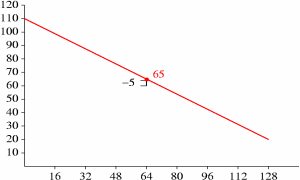
\includegraphics[width=8cm]{floor1-1}
\captionof{figure}{graph of example floor}
\end{center}

We now draw new logical lines to reflect the correction to new_Y, and
iterate for X positions 32 and 96:

\begin{center}
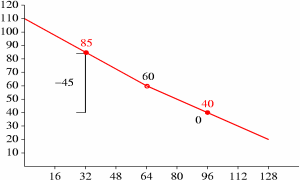
\includegraphics[width=8cm]{floor1-2}
\captionof{figure}{graph of example floor}
\end{center}

Although the new Y value at X position 96 is unchanged, it is still
used later as an endpoint for further refinement.  From here on, the
pattern should be clear; we complete the floor computation as follows:

\begin{center}
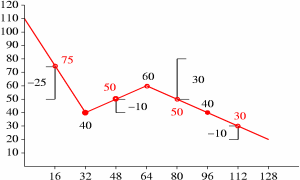
\includegraphics[width=8cm]{floor1-3}
\captionof{figure}{graph of example floor}
\end{center}

\begin{center}
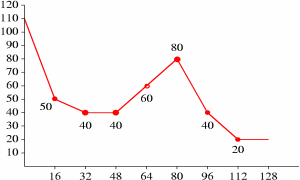
\includegraphics[width=8cm]{floor1-4}
\captionof{figure}{graph of example floor}
\end{center}

A more efficient algorithm with carefully defined integer rounding
behavior is used for actual decode, as described later.  The actual
algorithm splits Y value computation and line plotting into two steps
with modifications to the above algorithm to eliminate noise
accumulation through integer roundoff/truncation.



\subsubsection{header decode}

A list of floor X values is stored in the packet header in interleaved
format (used in list order during packet decode and synthesis).  This
list is split into partitions, and each partition is assigned to a
partition class.  X positions 0 and [n] are implicit and do not belong
to an explicit partition or partition class.

A partition class consists of a representation vector width (the
number of Y values which the partition class encodes at once), a
'subclass' value representing the number of alternate entropy books
the partition class may use in representing Y values, the list of
[subclass] books and a master book used to encode which alternate
books were chosen for representation in a given packet.  The
master/subclass mechanism is meant to be used as a flexible
representation cascade while still using codebooks only in a scalar
context.

\begin{Verbatim}[commandchars=\\\{\}]

  1) [floor1\_partitions] = read 5 bits as unsigned integer
  2) [maximum\_class] = -1
  3) iterate [i] over the range 0 ... [floor1\_partitions]-1 \{

        4) vector [floor1\_partition\_class\_list] element [i] = read 4 bits as unsigned integer

     \}

  5) [maximum\_class] = largest integer scalar value in vector [floor1\_partition\_class\_list]
  6) iterate [i] over the range 0 ... [maximum\_class] \{

        7) vector [floor1\_class\_dimensions] element [i] = read 3 bits as unsigned integer and add 1
	8) vector [floor1\_class\_subclasses] element [i] = read 2 bits as unsigned integer
        9) if ( vector [floor1\_class\_subclasses] element [i] is nonzero ) \{

             10) vector [floor1\_class\_masterbooks] element [i] = read 8 bits as unsigned integer

           \}

       11) iterate [j] over the range 0 ... (2 exponent [floor1\_class\_subclasses] element [i]) - 1 \{

             12) array [floor1\_subclass\_books] element [i],[j] =
                 read 8 bits as unsigned integer and subtract one
           \}
      \}

 13) [floor1\_multiplier] = read 2 bits as unsigned integer and add one
 14) [rangebits] = read 4 bits as unsigned integer
 15) vector [floor1\_X\_list] element [0] = 0
 16) vector [floor1\_X\_list] element [1] = 2 exponent [rangebits];
 17) [floor1\_values] = 2
 18) iterate [i] over the range 0 ... [floor1\_partitions]-1 \{

       19) [current\_class\_number] = vector [floor1\_partition\_class\_list] element [i]
       20) iterate [j] over the range 0 ... ([floor1\_class\_dimensions] element [current\_class\_number])-1 \{
             21) vector [floor1\_X\_list] element ([floor1\_values]) =
                 read [rangebits] bits as unsigned integer
             22) increment [floor1\_values] by one
           \}
     \}

 23) done
\end{Verbatim}

An end-of-packet condition while reading any aspect of a floor 1
configuration during setup renders a stream undecodable.  In addition,
a \varname{[floor1\_class\_masterbooks]} or
\varname{[floor1\_subclass\_books]} scalar element greater than the
highest numbered codebook configured in this stream is an error
condition that renders the stream undecodable.  Vector
[floor1\_x\_list] is limited to a maximum length of 65 elements; a
setup indicating more than 65 total elements (including elements 0 and
1 set prior to the read loop) renders the stream undecodable.  All
vector [floor1\_x\_list] element values must be unique within the
vector; a non-unique value renders the stream undecodable.

\subsubsection{packet decode} \label{vorbis:spec:floor1-decode}

Packet decode begins by checking the \varname{[nonzero]} flag:

\begin{Verbatim}[commandchars=\\\{\}]
  1) [nonzero] = read 1 bit as boolean
\end{Verbatim}

If \varname{[nonzero]} is unset, that indicates this channel contained
no audio energy in this frame.  Decode immediately returns a status
indicating this floor curve (and thus this channel) is unused this
frame.  (A return status of 'unused' is different from decoding a
floor that has all points set to minimum representation amplitude,
which happens to be approximately -140dB).


Assuming \varname{[nonzero]} is set, decode proceeds as follows:

\begin{Verbatim}[commandchars=\\\{\}]
  1) [range] = vector \{ 256, 128, 86, 64 \} element ([floor1\_multiplier]-1)
  2) vector [floor1\_Y] element [0] = read \link{vorbis:spec:ilog}{ilog}([range]-1) bits as unsigned integer
  3) vector [floor1\_Y] element [1] = read \link{vorbis:spec:ilog}{ilog}([range]-1) bits as unsigned integer
  4) [offset] = 2;
  5) iterate [i] over the range 0 ... [floor1\_partitions]-1 \{

       6) [class] = vector [floor1\_partition\_class]  element [i]
       7) [cdim]  = vector [floor1\_class\_dimensions] element [class]
       8) [cbits] = vector [floor1\_class\_subclasses] element [class]
       9) [csub]  = (2 exponent [cbits])-1
      10) [cval]  = 0
      11) if ( [cbits] is greater than zero ) \{

             12) [cval] = read from packet using codebook number
                 (vector [floor1\_class\_masterbooks] element [class]) in scalar context
          \}

      13) iterate [j] over the range 0 ... [cdim]-1 \{

             14) [book] = array [floor1\_subclass\_books] element [class],([cval] bitwise AND [csub])
             15) [cval] = [cval] right shifted [cbits] bits
	     16) if ( [book] is not less than zero ) \{

	           17) vector [floor1\_Y] element ([j]+[offset]) = read from packet using codebook
                       [book] in scalar context

                 \} else [book] is less than zero \{

	           18) vector [floor1\_Y] element ([j]+[offset]) = 0

                 \}
          \}

      19) [offset] = [offset] + [cdim]

     \}

 20) done
\end{Verbatim}

An end-of-packet condition during curve decode should be considered a
nominal occurrence; if end-of-packet is reached during any read
operation above, floor decode is to return 'unused' status as if the
\varname{[nonzero]} flag had been unset at the beginning of decode.


Vector \varname{[floor1\_Y]} contains the values from packet decode
needed for floor 1 synthesis.



\subsubsection{curve computation} \label{vorbis:spec:floor1-synth}

Curve computation is split into two logical steps; the first step
derives final Y amplitude values from the encoded, wrapped difference
values taken from the bitstream.  The second step plots the curve
lines.  Also, although zero-difference values are used in the
iterative prediction to find final Y values, these points are
conditionally skipped during final line computation in step two.
Skipping zero-difference values allows a smoother line fit.

Although some aspects of the below algorithm look like inconsequential
optimizations, implementors are warned to follow the details closely.
Deviation from implementing a strictly equivalent algorithm can result
in serious decoding errors.

{\em Additional note:} Although \varname{[floor1\_final\_Y]} values in
the prediction loop and at the end of step 1 are inherently limited by
the prediction algorithm to [0, \varname{[range]}), it is possible to
  abuse the setup and codebook machinery to produce negative or
  over-range results.  We suggest that decoder implementations guard
  the values in vector \varname{[floor1\_final\_Y]} by clamping each
  element to [0, \varname{[range]}) after step 1.  Variants of this
    suggestion are acceptable as valid floor1 setups cannot produce
    out of range values.

\begin{description}
\item[step 1: amplitude value synthesis]

Unwrap the always-positive-or-zero values read from the packet into
+/- difference values, then apply to line prediction.

\begin{Verbatim}[commandchars=\\\{\}]
  1) [range] = vector \{ 256, 128, 86, 64 \} element ([floor1\_multiplier]-1)
  2) vector [floor1\_step2\_flag] element [0] = set
  3) vector [floor1\_step2\_flag] element [1] = set
  4) vector [floor1\_final\_Y] element [0] = vector [floor1\_Y] element [0]
  5) vector [floor1\_final\_Y] element [1] = vector [floor1\_Y] element [1]
  6) iterate [i] over the range 2 ... [floor1\_values]-1 \{

       7) [low\_neighbor\_offset] = \link{vorbis:spec:low:neighbor}{low\_neighbor}([floor1\_X\_list],[i])
       8) [high\_neighbor\_offset] = \link{vorbis:spec:high:neighbor}{high\_neighbor}([floor1\_X\_list],[i])

       9) [predicted] = \link{vorbis:spec:render:point}{render\_point}( vector [floor1\_X\_list] element [low\_neighbor\_offset],
				      vector [floor1\_final\_Y] element [low\_neighbor\_offset],
                                      vector [floor1\_X\_list] element [high\_neighbor\_offset],
				      vector [floor1\_final\_Y] element [high\_neighbor\_offset],
                                      vector [floor1\_X\_list] element [i] )

      10) [val] = vector [floor1\_Y] element [i]
      11) [highroom] = [range] - [predicted]
      12) [lowroom]  = [predicted]
      13) if ( [highroom] is less than [lowroom] ) \{

            14) [room] = [highroom] * 2

          \} else [highroom] is not less than [lowroom] \{

            15) [room] = [lowroom] * 2

          \}

      16) if ( [val] is nonzero ) \{

            17) vector [floor1\_step2\_flag] element [low\_neighbor\_offset] = set
            18) vector [floor1\_step2\_flag] element [high\_neighbor\_offset] = set
            19) vector [floor1\_step2\_flag] element [i] = set
            20) if ( [val] is greater than or equal to [room] ) \{

                  21) if ( [highroom] is greater than [lowroom] ) \{

                        22) vector [floor1\_final\_Y] element [i] = [val] - [lowroom] + [predicted]

		      \} else [highroom] is not greater than [lowroom] \{

                        23) vector [floor1\_final\_Y] element [i] = [predicted] - [val] + [highroom] - 1

                      \}

                \} else [val] is less than [room] \{

                    24) if ([val] is odd) \{

                        25) vector [floor1\_final\_Y] element [i] =
                            [predicted] - (([val] + 1) divided by  2 using integer division)

                      \} else [val] is even \{

                        26) vector [floor1\_final\_Y] element [i] =
                            [predicted] + ([val] / 2 using integer division)

                      \}

                \}

          \} else [val] is zero \{

            27) vector [floor1\_step2\_flag] element [i] = unset
            28) vector [floor1\_final\_Y] element [i] = [predicted]

          \}

     \}

 29) done

\end{Verbatim}



\item[step 2: curve synthesis]

Curve synthesis generates a return vector \varname{[floor]} of length
\varname{[n]} (where \varname{[n]} is provided by the decode process
calling to floor decode).  Floor 1 curve synthesis makes use of the
\varname{[floor1\_X\_list]}, \varname{[floor1\_final\_Y]} and
\varname{[floor1\_step2\_flag]} vectors, as well as [floor1\_multiplier]
and [floor1\_values] values.

Decode begins by sorting the scalars from vectors
\varname{[floor1\_X\_list]}, \varname{[floor1\_final\_Y]} and
\varname{[floor1\_step2\_flag]} together into new vectors
\varname{[floor1\_X\_list]'}, \varname{[floor1\_final\_Y]'} and
\varname{[floor1\_step2\_flag]'} according to ascending sort order of the
values in \varname{[floor1\_X\_list]}.  That is, sort the values of
\varname{[floor1\_X\_list]} and then apply the same permutation to
elements of the other two vectors so that the X, Y and step2\_flag
values still match.

Then compute the final curve in one pass:

\begin{Verbatim}[commandchars=\\\{\}]
  1) [hx] = 0
  2) [lx] = 0
  3) [ly] = vector [floor1\_final\_Y]' element [0] * [floor1\_multiplier]
  4) iterate [i] over the range 1 ... [floor1\_values]-1 \{

       5) if ( [floor1\_step2\_flag]' element [i] is set ) \{

             6) [hy] = [floor1\_final\_Y]' element [i] * [floor1\_multiplier]
 	     7) [hx] = [floor1\_X\_list]' element [i]
             8) \link{vorbis:spec:render:line}{render\_line}( [lx], [ly], [hx], [hy], [floor] )
             9) [lx] = [hx]
	    10) [ly] = [hy]
          \}
     \}

 11) if ( [hx] is less than [n] ) \{

        12) \link{vorbis:spec:render:line}{render\_line}( [hx], [hy], [n], [hy], [floor] )

     \}

 13) if ( [hx] is greater than [n] ) \{

            14) truncate vector [floor] to [n] elements

     \}

 15) for each scalar in vector [floor], perform a lookup substitution using
     the scalar value from [floor] as an offset into the vector \link{vorbis:spec:floor1:inverse:dB:table}{[floor1\_inverse\_dB\_static\_table]}

 16) done

\end{Verbatim}

\end{description}

% -*- mode: latex; TeX-master: "Vorbis_I_spec"; -*-
%!TEX root = Vorbis_I_spec.tex
% $Id$
\section{Residue setup and decode} \label{vorbis:spec:residue}

\subsection{Overview}

A residue vector represents the fine detail of the audio spectrum of
one channel in an audio frame after the encoder subtracts the floor
curve and performs any channel coupling.  A residue vector may
represent spectral lines, spectral magnitude, spectral phase or
hybrids as mixed by channel coupling.  The exact semantic content of
the vector does not matter to the residue abstraction.

Whatever the exact qualities, the Vorbis residue abstraction codes the
residue vectors into the bitstream packet, and then reconstructs the
vectors during decode.  Vorbis makes use of three different encoding
variants (numbered 0, 1 and 2) of the same basic vector encoding
abstraction.



\subsection{Residue format}

Residue format partitions each vector in the vector bundle into chunks,
classifies each chunk, encodes the chunk classifications and finally
encodes the chunks themselves using the the specific VQ arrangement
defined for each selected classification.
The exact interleaving and partitioning vary by residue encoding number,
however the high-level process used to classify and encode the residue
vector is the same in all three variants.

A set of coded residue vectors are all of the same length.  High level
coding structure, ignoring for the moment exactly how a partition is
encoded and simply trusting that it is, is as follows:

\begin{itemize}
\item Each vector is partitioned into multiple equal sized chunks
according to configuration specified.  If we have a vector size of
\emph{n}, a partition size \emph{residue\_partition\_size}, and a total
of \emph{ch} residue vectors, the total number of partitioned chunks
coded is \emph{n}/\emph{residue\_partition\_size}*\emph{ch}.  It is
important to note that the integer division truncates.  In the below
example, we assume an example \emph{residue\_partition\_size} of 8.

\item Each partition in each vector has a classification number that
specifies which of multiple configured VQ codebook setups are used to
decode that partition.  The classification numbers of each partition
can be thought of as forming a vector in their own right, as in the
illustration below.  Just as the residue vectors are coded in grouped
partitions to increase encoding efficiency, the classification vector
is also partitioned into chunks.  The integer elements of each scalar
in a classification chunk are built into a single scalar that
represents the classification numbers in that chunk.  In the below
example, the classification codeword encodes two classification
numbers.

\item The values in a residue vector may be encoded monolithically in a
single pass through the residue vector, but more often efficient
codebook design dictates that each vector is encoded as the additive
sum of several passes through the residue vector using more than one
VQ codebook.  Thus, each residue value potentially accumulates values
from multiple decode passes.  The classification value associated with
a partition is the same in each pass, thus the classification codeword
is coded only in the first pass.

\end{itemize}


\begin{center}
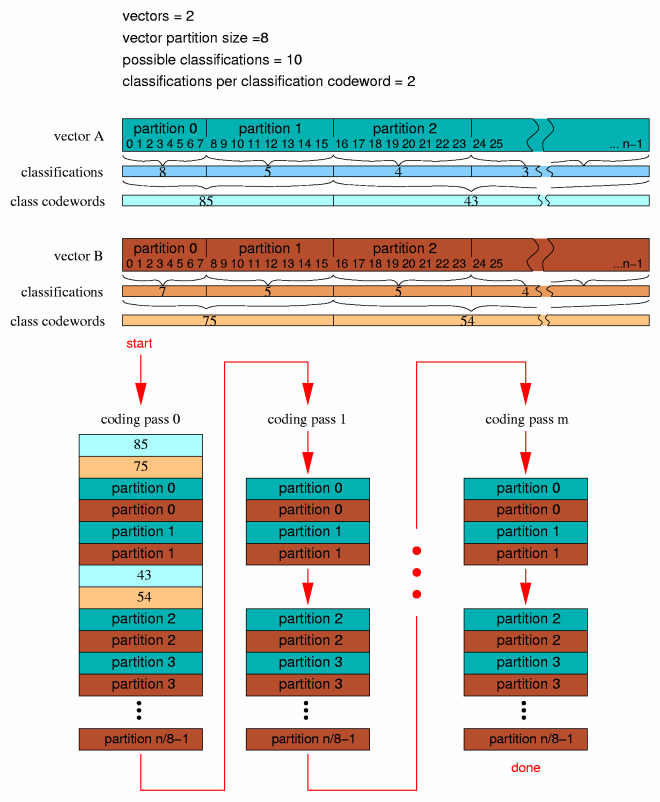
\includegraphics[width=\textwidth]{residue-pack}
\captionof{figure}{illustration of residue vector format}
\end{center}



\subsection{residue 0}

Residue 0 and 1 differ only in the way the values within a residue
partition are interleaved during partition encoding (visually treated
as a black box--or cyan box or brown box--in the above figure).

Residue encoding 0 interleaves VQ encoding according to the
dimension of the codebook used to encode a partition in a specific
pass.  The dimension of the codebook need not be the same in multiple
passes, however the partition size must be an even multiple of the
codebook dimension.

As an example, assume a partition vector of size eight, to be encoded
by residue 0 using codebook sizes of 8, 4, 2 and 1:

\begin{programlisting}

            original residue vector: [ 0 1 2 3 4 5 6 7 ]

codebook dimensions = 8  encoded as: [ 0 1 2 3 4 5 6 7 ]

codebook dimensions = 4  encoded as: [ 0 2 4 6 ], [ 1 3 5 7 ]

codebook dimensions = 2  encoded as: [ 0 4 ], [ 1 5 ], [ 2 6 ], [ 3 7 ]

codebook dimensions = 1  encoded as: [ 0 ], [ 1 ], [ 2 ], [ 3 ], [ 4 ], [ 5 ], [ 6 ], [ 7 ]

\end{programlisting}

It is worth mentioning at this point that no configurable value in the
residue coding setup is restricted to a power of two.



\subsection{residue 1}

Residue 1 does not interleave VQ encoding.  It represents partition
vector scalars in order.  As with residue 0, however, partition length
must be an integer multiple of the codebook dimension, although
dimension may vary from pass to pass.

As an example, assume a partition vector of size eight, to be encoded
by residue 0 using codebook sizes of 8, 4, 2 and 1:

\begin{programlisting}

            original residue vector: [ 0 1 2 3 4 5 6 7 ]

codebook dimensions = 8  encoded as: [ 0 1 2 3 4 5 6 7 ]

codebook dimensions = 4  encoded as: [ 0 1 2 3 ], [ 4 5 6 7 ]

codebook dimensions = 2  encoded as: [ 0 1 ], [ 2 3 ], [ 4 5 ], [ 6 7 ]

codebook dimensions = 1  encoded as: [ 0 ], [ 1 ], [ 2 ], [ 3 ], [ 4 ], [ 5 ], [ 6 ], [ 7 ]

\end{programlisting}



\subsection{residue 2}

Residue type two can be thought of as a variant of residue type 1.
Rather than encoding multiple passed-in vectors as in residue type 1,
the \emph{ch} passed in vectors of length \emph{n} are first
interleaved and flattened into a single vector of length
\emph{ch}*\emph{n}.  Encoding then proceeds as in type 1. Decoding is
as in type 1 with decode interleave reversed. If operating on a single
vector to begin with, residue type 1 and type 2 are equivalent.

\begin{center}
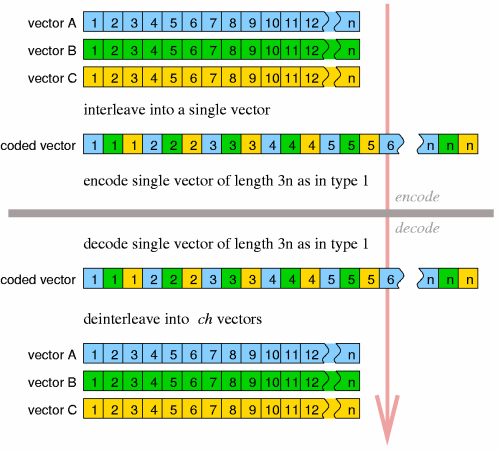
\includegraphics[width=\textwidth]{residue2}
\captionof{figure}{illustration of residue type 2}
\end{center}


\subsection{Residue decode}

\subsubsection{header decode}

Header decode for all three residue types is identical.
\begin{programlisting}
  1) [residue\_begin] = read 24 bits as unsigned integer
  2) [residue\_end] = read 24 bits as unsigned integer
  3) [residue\_partition\_size] = read 24 bits as unsigned integer and add one
  4) [residue\_classifications] = read 6 bits as unsigned integer and add one
  5) [residue\_classbook] = read 8 bits as unsigned integer
\end{programlisting}

\varname{[residue\_begin]} and
\varname{[residue\_end]} select the specific sub-portion of
each vector that is actually coded; it implements akin to a bandpass
where, for coding purposes, the vector effectively begins at element
\varname{[residue\_begin]} and ends at
\varname{[residue\_end]}.  Preceding and following values in
the unpacked vectors are zeroed.  Note that for residue type 2, these
values as well as \varname{[residue\_partition\_size]}apply to
the interleaved vector, not the individual vectors before interleave.
\varname{[residue\_partition\_size]} is as explained above,
\varname{[residue\_classifications]} is the number of possible
classification to which a partition can belong and
\varname{[residue\_classbook]} is the codebook number used to
code classification codewords.  The number of dimensions in book
\varname{[residue\_classbook]} determines how many
classification values are grouped into a single classification
codeword.  Note that the number of entries and dimensions in book
\varname{[residue\_classbook]}, along with
\varname{[residue\_classifications]}, overdetermines to
possible number of classification codewords.  
If \varname{[residue\_classifications]}\^{}\varname{[residue\_classbook]}.dimensions
exceeds \varname{[residue\_classbook]}.entries, the
bitstream should be regarded to be undecodable.

Next we read a bitmap pattern that specifies which partition classes
code values in which passes.

\begin{programlisting}
  1) iterate [i] over the range 0 ... [residue\_classifications]-1 {

       2) [high\_bits] = 0
       3) [low\_bits] = read 3 bits as unsigned integer
       4) [bitflag] = read one bit as boolean
       5) if ( [bitflag] is set ) then [high\_bits] = read five bits as unsigned integer
       6) vector [residue\_cascade] element [i] = [high\_bits] * 8 + [low\_bits]
     }
  7) done
\end{programlisting}

Finally, we read in a list of book numbers, each corresponding to
specific bit set in the cascade bitmap.  We loop over the possible
codebook classifications and the maximum possible number of encoding
stages (8 in Vorbis I, as constrained by the elements of the cascade
bitmap being eight bits):

\begin{programlisting}
  1) iterate [i] over the range 0 ... [residue\_classifications]-1 {

       2) iterate [j] over the range 0 ... 7 {

            3) if ( vector [residue\_cascade] element [i] bit [j] is set ) {

                 4) array [residue\_books] element [i][j] = read 8 bits as unsigned integer

               } else {

                 5) array [residue\_books] element [i][j] = unused

               }
          }
      }

  6) done
\end{programlisting}

An end-of-packet condition at any point in header decode renders the
stream undecodable.  In addition, any codebook number greater than the
maximum numbered codebook set up in this stream also renders the
stream undecodable. All codebooks in array [residue\_books] are
required to have a value mapping.  The presence of codebook in array
[residue\_books] without a value mapping (maptype equals zero) renders
the stream undecodable.



\subsubsection{packet decode}

Format 0 and 1 packet decode is identical except for specific
partition interleave.  Format 2 packet decode can be built out of the
format 1 decode process.  Thus we describe first the decode
infrastructure identical to all three formats.

In addition to configuration information, the residue decode process
is passed the number of vectors in the submap bundle and a vector of
flags indicating if any of the vectors are not to be decoded.  If the
passed in number of vectors is 3 and vector number 1 is marked 'do not
decode', decode skips vector 1 during the decode loop.  However, even
'do not decode' vectors are allocated and zeroed.

Depending on the values of \varname{[residue\_begin]} and
\varname{[residue\_end]}, it is obvious that the encoded
portion of a residue vector may be the entire possible residue vector
or some other strict subset of the actual residue vector size with
zero padding at either uncoded end.  However, it is also possible to
set \varname{[residue\_begin]} and
\varname{[residue\_end]} to specify a range partially or
wholly beyond the maximum vector size.  Before beginning residue
decode, limit \varname{[residue\_begin]} and
\varname{[residue\_end]} to the maximum possible vector size
as follows.  We assume that the number of vectors being encoded,
\varname{[ch]} is provided by the higher level decoding
process.

\begin{programlisting}
  1) [actual\_size] = current blocksize/2;
  2) if residue encoding is format 2
       3) [actual\_size] = [actual\_size] * [ch];
  4) [limit\_residue\_begin] = maximum of ([residue\_begin],[actual\_size]);
  5) [limit\_residue\_end] = maximum of ([residue\_end],[actual\_size]);
\end{programlisting}

The following convenience values are conceptually useful to clarifying
the decode process:

\begin{programlisting}
  1) [classwords\_per\_codeword] = [codebook\_dimensions] value of codebook [residue\_classbook]
  2) [n\_to\_read] = [limit\_residue\_end] - [limit\_residue\_begin]
  3) [partitions\_to\_read] = [n\_to\_read] / [residue\_partition\_size]
\end{programlisting}

Packet decode proceeds as follows, matching the description offered earlier in the document.
\begin{programlisting}
  1) allocate and zero all vectors that will be returned.
  2) if ([n\_to\_read] is zero), stop; there is no residue to decode.
  3) iterate [pass] over the range 0 ... 7 {

       4) [partition\_count] = 0

       5) while [partition\_count] is less than [partitions\_to\_read]

            6) if ([pass] is zero) {

                 7) iterate [j] over the range 0 .. [ch]-1 {

                      8) if vector [j] is not marked 'do not decode' {

                           9) [temp] = read from packet using codebook [residue\_classbook] in scalar context
                          10) iterate [i] descending over the range [classwords\_per\_codeword]-1 ... 0 {

                               11) array [classifications] element [j],([i]+[partition\_count]) =
                                   [temp] integer modulo [residue\_classifications]
                               12) [temp] = [temp] / [residue\_classifications] using integer division

                              }

                         }

                    }

               }

           13) iterate [i] over the range 0 .. ([classwords\_per\_codeword] - 1) while [partition\_count]
               is also less than [partitions\_to\_read] {

                 14) iterate [j] over the range 0 .. [ch]-1 {

                      15) if vector [j] is not marked 'do not decode' {

                           16) [vqclass] = array [classifications] element [j],[partition\_count]
                           17) [vqbook] = array [residue\_books] element [vqclass],[pass]
                           18) if ([vqbook] is not 'unused') {

                                19) decode partition into output vector number [j], starting at scalar
                                    offset [limit\_residue\_begin]+[partition\_count]*[residue\_partition\_size] using
                                    codebook number [vqbook] in VQ context
                          }
                     }

                 20) increment [partition\_count] by one

               }
          }
     }

 21) done

\end{programlisting}

An end-of-packet condition during packet decode is to be considered a
nominal occurrence.  Decode returns the result of vector decode up to
that point.



\subsubsection{format 0 specifics}

Format zero decodes partitions exactly as described earlier in the
'Residue Format: residue 0' section.  The following pseudocode
presents the same algorithm. Assume:

\begin{itemize}
\item  \varname{[n]} is the value in \varname{[residue\_partition\_size]}
\item \varname{[v]} is the residue vector
\item \varname{[offset]} is the beginning read offset in [v]
\end{itemize}


\begin{programlisting}
 1) [step] = [n] / [codebook\_dimensions]
 2) iterate [i] over the range 0 ... [step]-1 {

      3) vector [entry\_temp] = read vector from packet using current codebook in VQ context
      4) iterate [j] over the range 0 ... [codebook\_dimensions]-1 {

           5) vector [v] element ([offset]+[i]+[j]*[step]) =
	        vector [v] element ([offset]+[i]+[j]*[step]) +
                vector [entry\_temp] element [j]

         }

    }

  6) done

\end{programlisting}



\subsubsection{format 1 specifics}

Format 1 decodes partitions exactly as described earlier in the
'Residue Format: residue 1' section.  The following pseudocode
presents the same algorithm. Assume:

\begin{itemize}
\item  \varname{[n]} is the value in
\varname{[residue\_partition\_size]}
\item \varname{[v]} is the residue vector
\item \varname{[offset]} is the beginning read offset in [v]
\end{itemize}


\begin{programlisting}
 1) [i] = 0
 2) vector [entry\_temp] = read vector from packet using current codebook in VQ context
 3) iterate [j] over the range 0 ... [codebook\_dimensions]-1 {

      4) vector [v] element ([offset]+[i]) =
	  vector [v] element ([offset]+[i]) +
          vector [entry\_temp] element [j]
      5) increment [i]

    }

  6) if ( [i] is less than [n] ) continue at step 2
  7) done
\end{programlisting}



\subsubsection{format 2 specifics}

Format 2 is reducible to format 1.  It may be implemented as an additional step prior to and an additional post-decode step after a normal format 1 decode.


Format 2 handles 'do not decode' vectors differently than residue 0 or
1; if all vectors are marked 'do not decode', no decode occurrs.
However, if at least one vector is to be decoded, all the vectors are
decoded.  We then request normal format 1 to decode a single vector
representing all output channels, rather than a vector for each
channel.  After decode, deinterleave the vector into independent vectors, one for each output channel.  That is:

\begin{enumerate}
 \item If all vectors 0 through \emph{ch}-1 are marked 'do not decode', allocate and clear a single vector \varname{[v]}of length \emph{ch*n} and skip step 2 below; proceed directly to the post-decode step.
 \item Rather than performing format 1 decode to produce \emph{ch} vectors of length \emph{n} each, call format 1 decode to produce a single vector \varname{[v]} of length \emph{ch*n}.
 \item Post decode: Deinterleave the single vector \varname{[v]} returned by format 1 decode as described above into \emph{ch} independent vectors, one for each outputchannel, according to:
  \begin{programlisting}
  1) iterate [i] over the range 0 ... [n]-1 {

       2) iterate [j] over the range 0 ... [ch]-1 {

            3) output vector number [j] element [i] = vector [v] element ([i] * [ch] + [j])

          }
     }

  4) done
  \end{programlisting}

\end{enumerate}








% -*- mode: latex; TeX-master: "Vorbis_I_spec"; -*-
%!TEX root = Vorbis_I_spec.tex
% $Id$
\section{Helper equations} \label{vorbis:spec:helper}

\subsection{Overview}

The equations below are used in multiple places by the Vorbis codec
specification.  Rather than cluttering up the main specification
documents, they are defined here and referenced where appropriate.


\subsection{Functions}

\subsubsection{ilog} \label{vorbis:spec:ilog}

The "ilog(x)" function returns the position number (1 through n) of the highest set bit in the two's complement integer value
\varname{[x]}.  Values of \varname{[x]} less than zero are defined to return zero.

\begin{programlisting}
  1) [return\_value] = 0;
  2) if ( [x] is greater than zero ) {

       3) increment [return\_value];
       4) logical shift [x] one bit to the right, padding the MSb with zero
       5) repeat at step 2)

     }

   6) done
\end{programlisting}

Examples:

\begin{itemize}
 \item ilog(0) = 0;
 \item ilog(1) = 1;
 \item ilog(2) = 2;
 \item ilog(3) = 2;
 \item ilog(4) = 3;
 \item ilog(7) = 3;
 \item ilog(negative number) = 0;
\end{itemize}




\subsubsection{float32\_unpack} \label{vorbis:spec:float32:unpack}

"float32\_unpack(x)" is intended to translate the packed binary
representation of a Vorbis codebook float value into the
representation used by the decoder for floating point numbers.  For
purposes of this example, we will unpack a Vorbis float32 into a
host-native floating point number.

\begin{programlisting}
  1) [mantissa] = [x] bitwise AND 0x1fffff (unsigned result)
  2) [sign] = [x] bitwise AND 0x80000000 (unsigned result)
  3) [exponent] = ( [x] bitwise AND 0x7fe00000) shifted right 21 bits (unsigned result)
  4) if ( [sign] is nonzero ) then negate [mantissa]
  5) return [mantissa] * ( 2 ^ ( [exponent] - 788 ) )
\end{programlisting}



\subsubsection{lookup1\_values} \label{vorbis:spec:lookup1:values}

"lookup1\_values(codebook\_entries,codebook\_dimensions)" is used to
compute the correct length of the value index for a codebook VQ lookup
table of lookup type 1.  The values on this list are permuted to
construct the VQ vector lookup table of size
\varname{[codebook\_entries]}.

The return value for this function is defined to be 'the greatest
integer value for which \varname{[return\_value]} to the power of
\varname{[codebook\_dimensions]} is less than or equal to
\varname{[codebook\_entries]}'.



\subsubsection{low\_neighbor} \label{vorbis:spec:low:neighbor}

"low\_neighbor(v,x)" finds the position \varname{n} in vector \varname{[v]} of
the greatest value scalar element for which \varname{n} is less than
\varname{[x]} and vector \varname{[v]} element \varname{n} is less
than vector \varname{[v]} element \varname{[x]}.

\subsubsection{high\_neighbor} \label{vorbis:spec:high:neighbor}

"high\_neighbor(v,x)" finds the position \varname{n} in vector [v] of
the lowest value scalar element for which \varname{n} is less than
\varname{[x]} and vector \varname{[v]} element \varname{n} is greater
than vector \varname{[v]} element \varname{[x]}.



\subsubsection{render\_point} \label{vorbis:spec:render:point}

"render\_point(x0,y0,x1,y1,X)" is used to find the Y value at point X
along the line specified by x0, x1, y0 and y1.  This function uses an
integer algorithm to solve for the point directly without calculating
intervening values along the line.

\begin{programlisting}
  1)  [dy] = [y1] - [y0]
  2) [adx] = [x1] - [x0]
  3) [ady] = absolute value of [dy]
  4) [err] = [ady] * ([X] - [x0])
  5) [off] = [err] / [adx] using integer division
  6) if ( [dy] is less than zero ) {

       7) [Y] = [y0] - [off]

     } else {

       8) [Y] = [y0] + [off]

     }

  9) done
\end{programlisting}



\subsubsection{render\_line} \label{vorbis:spec:render:line}

Floor decode type one uses the integer line drawing algorithm of
"render\_line(x0, y0, x1, y1, v)" to construct an integer floor
curve for contiguous piecewise line segments. Note that it has not
been relevant elsewhere, but here we must define integer division as
rounding division of both positive and negative numbers toward zero.


\begin{programlisting}
  1)   [dy] = [y1] - [y0]
  2)  [adx] = [x1] - [x0]
  3)  [ady] = absolute value of [dy]
  4) [base] = [dy] / [adx] using integer division
  5)    [x] = [x0]
  6)    [y] = [y0]
  7)  [err] = 0

  8) if ( [dy] is less than 0 ) {

        9) [sy] = [base] - 1

     } else {

       10) [sy] = [base] + 1

     }

 11) [ady] = [ady] - (absolute value of [base]) * [adx]
 12) vector [v] element [x] = [y]

 13) iterate [x] over the range [x0]+1 ... [x1]-1 {

       14) [err] = [err] + [ady];
       15) if ( [err] >= [adx] ) {

             16) [err] = [err] - [adx]
             17)   [y] = [y] + [sy]

           } else {

             18) [y] = [y] + [base]

           }

       19) vector [v] element [x] = [y]

     }
\end{programlisting}









% -*- mode: latex; TeX-master: "Vorbis_I_spec"; -*-
%!TEX root = Vorbis_I_spec.tex
% $Id$
\section{Tables} \label{vorbis:spec:tables}

\subsection{floor1\_inverse\_dB\_table} \label{vorbis:spec:floor1:inverse:dB:table}

The vector \varname{[floor1\_inverse\_dB\_table]} is a 256 element static
lookup table consiting of the following values (read left to right
then top to bottom):

\begin{Verbatim}
  1.0649863e-07, 1.1341951e-07, 1.2079015e-07, 1.2863978e-07,
  1.3699951e-07, 1.4590251e-07, 1.5538408e-07, 1.6548181e-07,
  1.7623575e-07, 1.8768855e-07, 1.9988561e-07, 2.1287530e-07,
  2.2670913e-07, 2.4144197e-07, 2.5713223e-07, 2.7384213e-07,
  2.9163793e-07, 3.1059021e-07, 3.3077411e-07, 3.5226968e-07,
  3.7516214e-07, 3.9954229e-07, 4.2550680e-07, 4.5315863e-07,
  4.8260743e-07, 5.1396998e-07, 5.4737065e-07, 5.8294187e-07,
  6.2082472e-07, 6.6116941e-07, 7.0413592e-07, 7.4989464e-07,
  7.9862701e-07, 8.5052630e-07, 9.0579828e-07, 9.6466216e-07,
  1.0273513e-06, 1.0941144e-06, 1.1652161e-06, 1.2409384e-06,
  1.3215816e-06, 1.4074654e-06, 1.4989305e-06, 1.5963394e-06,
  1.7000785e-06, 1.8105592e-06, 1.9282195e-06, 2.0535261e-06,
  2.1869758e-06, 2.3290978e-06, 2.4804557e-06, 2.6416497e-06,
  2.8133190e-06, 2.9961443e-06, 3.1908506e-06, 3.3982101e-06,
  3.6190449e-06, 3.8542308e-06, 4.1047004e-06, 4.3714470e-06,
  4.6555282e-06, 4.9580707e-06, 5.2802740e-06, 5.6234160e-06,
  5.9888572e-06, 6.3780469e-06, 6.7925283e-06, 7.2339451e-06,
  7.7040476e-06, 8.2047000e-06, 8.7378876e-06, 9.3057248e-06,
  9.9104632e-06, 1.0554501e-05, 1.1240392e-05, 1.1970856e-05,
  1.2748789e-05, 1.3577278e-05, 1.4459606e-05, 1.5399272e-05,
  1.6400004e-05, 1.7465768e-05, 1.8600792e-05, 1.9809576e-05,
  2.1096914e-05, 2.2467911e-05, 2.3928002e-05, 2.5482978e-05,
  2.7139006e-05, 2.8902651e-05, 3.0780908e-05, 3.2781225e-05,
  3.4911534e-05, 3.7180282e-05, 3.9596466e-05, 4.2169667e-05,
  4.4910090e-05, 4.7828601e-05, 5.0936773e-05, 5.4246931e-05,
  5.7772202e-05, 6.1526565e-05, 6.5524908e-05, 6.9783085e-05,
  7.4317983e-05, 7.9147585e-05, 8.4291040e-05, 8.9768747e-05,
  9.5602426e-05, 0.00010181521, 0.00010843174, 0.00011547824,
  0.00012298267, 0.00013097477, 0.00013948625, 0.00014855085,
  0.00015820453, 0.00016848555, 0.00017943469, 0.00019109536,
  0.00020351382, 0.00021673929, 0.00023082423, 0.00024582449,
  0.00026179955, 0.00027881276, 0.00029693158, 0.00031622787,
  0.00033677814, 0.00035866388, 0.00038197188, 0.00040679456,
  0.00043323036, 0.00046138411, 0.00049136745, 0.00052329927,
  0.00055730621, 0.00059352311, 0.00063209358, 0.00067317058,
  0.00071691700, 0.00076350630, 0.00081312324, 0.00086596457,
  0.00092223983, 0.00098217216, 0.0010459992,  0.0011139742,
  0.0011863665,  0.0012634633,  0.0013455702,  0.0014330129,
  0.0015261382,  0.0016253153,  0.0017309374,  0.0018434235,
  0.0019632195,  0.0020908006,  0.0022266726,  0.0023713743,
  0.0025254795,  0.0026895994,  0.0028643847,  0.0030505286,
  0.0032487691,  0.0034598925,  0.0036847358,  0.0039241906,
  0.0041792066,  0.0044507950,  0.0047400328,  0.0050480668,
  0.0053761186,  0.0057254891,  0.0060975636,  0.0064938176,
  0.0069158225,  0.0073652516,  0.0078438871,  0.0083536271,
  0.0088964928,  0.009474637,   0.010090352,   0.010746080,
  0.011444421,   0.012188144,   0.012980198,   0.013823725,
  0.014722068,   0.015678791,   0.016697687,   0.017782797,
  0.018938423,   0.020169149,   0.021479854,   0.022875735,
  0.024362330,   0.025945531,   0.027631618,   0.029427276,
  0.031339626,   0.033376252,   0.035545228,   0.037855157,
  0.040315199,   0.042935108,   0.045725273,   0.048696758,
  0.051861348,   0.055231591,   0.058820850,   0.062643361,
  0.066714279,   0.071049749,   0.075666962,   0.080584227,
  0.085821044,   0.091398179,   0.097337747,   0.10366330,
  0.11039993,    0.11757434,    0.12521498,    0.13335215,
  0.14201813,    0.15124727,    0.16107617,    0.17154380,
  0.18269168,    0.19456402,    0.20720788,    0.22067342,
  0.23501402,    0.25028656,    0.26655159,    0.28387361,
  0.30232132,    0.32196786,    0.34289114,    0.36517414,
  0.38890521,    0.41417847,    0.44109412,    0.46975890,
  0.50028648,    0.53279791,    0.56742212,    0.60429640,
  0.64356699,    0.68538959,    0.72993007,    0.77736504,
  0.82788260,    0.88168307,    0.9389798,     1.
\end{Verbatim}


\appendix
% -*- mode: latex; TeX-master: "Vorbis_I_spec"; -*-
%!TEX root = Vorbis_I_spec.tex
% $Id$
\section{Embedding Vorbis into an Ogg stream} \label{vorbis:over:ogg}

\subsection{Overview}

This document describes using Ogg logical and physical transport
streams to encapsulate Vorbis compressed audio packet data into file
form.

The \xref{vorbis:spec:intro} provides an overview of the construction
of Vorbis audio packets.

The \href{oggstream.html}{Ogg
bitstream overview} and \href{framing.html}{Ogg logical
bitstream and framing spec} provide detailed descriptions of Ogg
transport streams. This specification document assumes a working
knowledge of the concepts covered in these named backround
documents.  Please read them first.

\subsubsection{Restrictions}

The Ogg/Vorbis I specification currently dictates that Ogg/Vorbis
streams use Ogg transport streams in degenerate, unmultiplexed
form only. That is:

\begin{itemize}
 \item
  A meta-headerless Ogg file encapsulates the Vorbis I packets

 \item
  The Ogg stream may be chained, i.e., contain multiple, contigous logical streams (links).

 \item
  The Ogg stream must be unmultiplexed (only one stream, a Vorbis audio stream, per link)

\end{itemize}


This is not to say that it is not currently possible to multiplex
Vorbis with other media types into a multi-stream Ogg file.  At the
time this document was written, Ogg was becoming a popular container
for low-bitrate movies consisting of DivX video and Vorbis audio.
However, a 'Vorbis I audio file' is taken to imply Vorbis audio
existing alone within a degenerate Ogg stream.  A compliant 'Vorbis
audio player' is not required to implement Ogg support beyond the
specific support of Vorbis within a degenrate Ogg stream (naturally,
application authors are encouraged to support full multiplexed Ogg
handling).




\subsubsection{MIME type}

The MIME type of Ogg files depend on the context.  Specifically, complex
multimedia and applications should use \literal{application/ogg},
while visual media should use \literal{video/ogg}, and audio
\literal{audio/ogg}.  Vorbis data encapsulated in Ogg may appear
in any of those types.  RTP encapsulated Vorbis should use
\literal{audio/vorbis} + \literal{audio/vorbis-config}.


\subsection{Encapsulation}

Ogg encapsulation of a Vorbis packet stream is straightforward.

\begin{itemize}

\item
  The first Vorbis packet (the identification header), which
  uniquely identifies a stream as Vorbis audio, is placed alone in the
  first page of the logical Ogg stream.  This results in a first Ogg
  page of exactly 58 bytes at the very beginning of the logical stream.


\item
  This first page is marked 'beginning of stream' in the page flags.


\item
  The second and third vorbis packets (comment and setup
  headers) may span one or more pages beginning on the second page of
  the logical stream.  However many pages they span, the third header
  packet finishes the page on which it ends.  The next (first audio) packet
  must begin on a fresh page.


\item
  The granule position of these first pages containing only headers is zero.


\item
  The first audio packet of the logical stream begins a fresh Ogg page.


\item
  Packets are placed into ogg pages in order until the end of stream.


\item
  The last page is marked 'end of stream' in the page flags.


\item
  Vorbis packets may span page boundaries.


\item
  The granule position of pages containing Vorbis audio is in units
  of PCM audio samples (per channel; a stereo stream's granule position
  does not increment at twice the speed of a mono stream).


\item
  The granule position of a page represents the end PCM sample
  position of the last packet \emph{completed} on that
  page.  The 'last PCM sample' is the last complete sample returned by
  decode, not an internal sample awaiting lapping with a
  subsequent block.  A page that is entirely spanned by a single
  packet (that completes on a subsequent page) has no granule
  position, and the granule position is set to '-1'.


  Note that the last decoded (fully lapped) PCM sample from a packet
  is not necessarily the middle sample from that block. If, eg, the
  current Vorbis packet encodes a "long block" and the next Vorbis
  packet encodes a "short block", the last decodable sample from the
  current packet be at position (3*long\_block\_length/4) -
  (short\_block\_length/4).


\item
    The granule (PCM) position of the first page need not indicate
    that the stream started at position zero.  Although the granule
    position belongs to the last completed packet on the page and a
    valid granule position must be positive, by
    inference it may indicate that the PCM position of the beginning
    of audio is positive or negative.


  \begin{itemize}
    \item
        A positive starting value simply indicates that this stream begins at
        some positive time offset, potentially within a larger
        program. This is a common case when connecting to the middle
        of broadcast stream.

    \item
        A negative value indicates that
        output samples preceeding time zero should be discarded during
        decoding; this technique is used to allow sample-granularity
        editing of the stream start time of already-encoded Vorbis
        streams.  The number of samples to be discarded must not exceed
        the overlap-add span of the first two audio packets.

  \end{itemize}


    In both of these cases in which the initial audio PCM starting
    offset is nonzero, the second finished audio packet must flush the
    page on which it appears and the third packet begin a fresh page.
    This allows the decoder to always be able to perform PCM position
    adjustments before needing to return any PCM data from synthesis,
    resulting in correct positioning information without any aditional
    seeking logic.


  \begin{note}
    Failure to do so should, at worst, cause a
    decoder implementation to return incorrect positioning information
    for seeking operations at the very beginning of the stream.
  \end{note}


\item
  A granule position on the final page in a stream that indicates
  less audio data than the final packet would normally return is used to
  end the stream on other than even frame boundaries.  The difference
  between the actual available data returned and the declared amount
  indicates how many trailing samples to discard from the decoding
  process.

\end{itemize}

% -*- mode: latex; TeX-master: "Vorbis_I_spec"; -*-
%!TEX root = Vorbis_I_spec.tex
% $Id$
\section{Vorbis encapsulation in RTP} \label{vorbis:over:rtp}

% TODO: Include draft-rtp.xml somehow?

Please consult RFC 5215 \textit{``RTP Payload Format for Vorbis Encoded
    Audio''} for description of how to embed Vorbis audio in an RTP stream.


% -*- mode: latex; TeX-master: "Vorbis_I_spec"; -*-
%!TEX root = Vorbis_I_spec.tex
% $Id$
\section*{Colophon}


\includegraphics{xifish} \label{footer}
%\TODO{display xifish.pdf, [Xiph.Org logo]}


Ogg is a \href{http://www.xiph.org/}{Xiph.Org Foundation} effort
to protect essential tenets of Internet multimedia from corporate
hostage-taking; Open Source is the net's greatest tool to keep
everyone honest. See \href{http://www.xiph.org/about.html}{About
the Xiph.Org Foundation} for details.


Ogg Vorbis is the first Ogg audio CODEC.  Anyone may freely use and
distribute the Ogg and Vorbis specification, whether in a private,
public or corporate capacity.  However, the Xiph.Org Foundation and
the Ogg project (xiph.org) reserve the right to set the Ogg Vorbis
specification and certify specification compliance.

Xiph.Org's Vorbis software CODEC implementation is distributed under a
BSD-like license.  This does not restrict third parties from
distributing independent implementations of Vorbis software under
other licenses.

Ogg, Vorbis, Xiph.Org Foundation and their logos are trademarks (tm)
of the \href{http://www.xiph.org/}{Xiph.Org Foundation}.  These
pages are copyright (C) 1994-2007 Xiph.Org Foundation. All rights
reserved.

This document is set using \LaTeX.

 
% TODO: Use a bibliography, as in the example below?
\begin{thebibliography}{99} 
 
\bibitem{Sporer/Brandenburg/Edler} T.~Sporer, K.~Brandenburg and B.~Edler, 
The use of multirate filter banks for coding of high quality digital audio,
\url{http://www.iocon.com/resource/docs/ps/eusipco_corrected.ps}.


\end{thebibliography}

\end{document}
